\documentclass[a4paper,fleqn]{cas-sc}
%DIF LATEXDIFF DIFFERENCE FILE
%DIF DEL old.tex   Sat Mar 11 14:14:05 2023
%DIF ADD new.tex   Sat Mar 11 14:17:43 2023

\usepackage[authoryear]{natbib}
\usepackage{graphicx} 
\usepackage{float}
\usepackage{algorithm}  
\usepackage{algpseudocode}
\usepackage{color}
\usepackage{setspace}
\usepackage[nomarkers,figuresonly]{endfloat}

\usepackage{dirtree}
%DIF 13a13-14
\usepackage{listings} %DIF > 
\usepackage{siunitx} %DIF > 
%DIF -------

%DIF 14c16-17
%DIF < \newcommand{\colorComments}{black} 
%DIF -------
\usepackage{xcolor} %DIF > 
\usepackage{bm} %DIF > 
%DIF -------

%DIF 16a19-45
\definecolor{codegreen}{rgb}{0,0.6,0} %DIF > 
\definecolor{codegray}{rgb}{0.5,0.5,0.5} %DIF > 
\definecolor{codepurple}{rgb}{0.58,0,0.82} %DIF > 
\definecolor{backcolour}{rgb}{0.95,0.95,0.92} %DIF > 
 %DIF > 
\lstdefinestyle{mystyle}{ %DIF > 
    backgroundcolor=\color{backcolour},    %DIF > 
    commentstyle=\color{codegreen}, %DIF > 
    keywordstyle=\color{blue}, %DIF > 
    numberstyle=\tiny\color{codegray}, %DIF > 
    stringstyle=\color{codepurple}, %DIF > 
    basicstyle=\ttfamily\footnotesize, %DIF > 
    breakatwhitespace=false,          %DIF > 
    breaklines=true,                  %DIF > 
    captionpos=b,                     %DIF > 
    keepspaces=true,                  %DIF > 
    numbers=left,                     %DIF > 
    numbersep=5pt,                   %DIF > 
    showspaces=false,                 %DIF > 
    showstringspaces=false, %DIF > 
    showtabs=false,                   %DIF > 
    tabsize=4 %DIF > 
} %DIF > 
\lstset{style=mystyle} %DIF > 
 %DIF > 
\newcommand{\colorComments}{black}  %DIF > 
\newcommand{\vecmat}[1]{\bm #1} %DIF > 
%DIF -------
%%%Author definitions
\def\tsc#1{\csdef{#1}{\textsc{\lowercase{#1}}\xspace}}
\tsc{MS}
\tsc{AFO}
%%%

\usepackage{lineno}
\linenumbers 
%DIF PREAMBLE EXTENSION ADDED BY LATEXDIFF
%DIF UNDERLINE PREAMBLE %DIF PREAMBLE
\RequirePackage[normalem]{ulem} %DIF PREAMBLE
\RequirePackage{color}\definecolor{RED}{rgb}{1,0,0}\definecolor{BLUE}{rgb}{0,0,1} %DIF PREAMBLE
\providecommand{\DIFadd}[1]{{\protect\color{blue}\uwave{#1}}} %DIF PREAMBLE
\providecommand{\DIFdel}[1]{{\protect\color{red}\sout{#1}}}                      %DIF PREAMBLE
%DIF SAFE PREAMBLE %DIF PREAMBLE
\providecommand{\DIFaddbegin}{} %DIF PREAMBLE
\providecommand{\DIFaddend}{} %DIF PREAMBLE
\providecommand{\DIFdelbegin}{} %DIF PREAMBLE
\providecommand{\DIFdelend}{} %DIF PREAMBLE
\providecommand{\DIFmodbegin}{} %DIF PREAMBLE
\providecommand{\DIFmodend}{} %DIF PREAMBLE
%DIF FLOATSAFE PREAMBLE %DIF PREAMBLE
\providecommand{\DIFaddFL}[1]{\DIFadd{#1}} %DIF PREAMBLE
\providecommand{\DIFdelFL}[1]{\DIFdel{#1}} %DIF PREAMBLE
\providecommand{\DIFaddbeginFL}{} %DIF PREAMBLE
\providecommand{\DIFaddendFL}{} %DIF PREAMBLE
\providecommand{\DIFdelbeginFL}{} %DIF PREAMBLE
\providecommand{\DIFdelendFL}{} %DIF PREAMBLE
\newcommand{\DIFscaledelfig}{0.5}
%DIF HIGHLIGHTGRAPHICS PREAMBLE %DIF PREAMBLE
\RequirePackage{settobox} %DIF PREAMBLE
\RequirePackage{letltxmacro} %DIF PREAMBLE
\newsavebox{\DIFdelgraphicsbox} %DIF PREAMBLE
\newlength{\DIFdelgraphicswidth} %DIF PREAMBLE
\newlength{\DIFdelgraphicsheight} %DIF PREAMBLE
% store original definition of \includegraphics %DIF PREAMBLE
\LetLtxMacro{\DIFOincludegraphics}{\includegraphics} %DIF PREAMBLE
\newcommand{\DIFaddincludegraphics}[2][]{{\color{blue}\fbox{\DIFOincludegraphics[#1]{#2}}}} %DIF PREAMBLE
\newcommand{\DIFdelincludegraphics}[2][]{% %DIF PREAMBLE
\sbox{\DIFdelgraphicsbox}{\DIFOincludegraphics[#1]{#2}}% %DIF PREAMBLE
\settoboxwidth{\DIFdelgraphicswidth}{\DIFdelgraphicsbox} %DIF PREAMBLE
\settoboxtotalheight{\DIFdelgraphicsheight}{\DIFdelgraphicsbox} %DIF PREAMBLE
\scalebox{\DIFscaledelfig}{% %DIF PREAMBLE
\parbox[b]{\DIFdelgraphicswidth}{\usebox{\DIFdelgraphicsbox}\\[-\baselineskip] \rule{\DIFdelgraphicswidth}{0em}}\llap{\resizebox{\DIFdelgraphicswidth}{\DIFdelgraphicsheight}{% %DIF PREAMBLE
\setlength{\unitlength}{\DIFdelgraphicswidth}% %DIF PREAMBLE
\begin{picture}(1,1)% %DIF PREAMBLE
\thicklines\linethickness{2pt} %DIF PREAMBLE
{\color[rgb]{1,0,0}\put(0,0){\framebox(1,1){}}}% %DIF PREAMBLE
{\color[rgb]{1,0,0}\put(0,0){\line( 1,1){1}}}% %DIF PREAMBLE
{\color[rgb]{1,0,0}\put(0,1){\line(1,-1){1}}}% %DIF PREAMBLE
\end{picture}% %DIF PREAMBLE
}\hspace*{3pt}}} %DIF PREAMBLE
} %DIF PREAMBLE
\LetLtxMacro{\DIFOaddbegin}{\DIFaddbegin} %DIF PREAMBLE
\LetLtxMacro{\DIFOaddend}{\DIFaddend} %DIF PREAMBLE
\LetLtxMacro{\DIFOdelbegin}{\DIFdelbegin} %DIF PREAMBLE
\LetLtxMacro{\DIFOdelend}{\DIFdelend} %DIF PREAMBLE
\DeclareRobustCommand{\DIFaddbegin}{\DIFOaddbegin \let\includegraphics\DIFaddincludegraphics} %DIF PREAMBLE
\DeclareRobustCommand{\DIFaddend}{\DIFOaddend \let\includegraphics\DIFOincludegraphics} %DIF PREAMBLE
\DeclareRobustCommand{\DIFdelbegin}{\DIFOdelbegin \let\includegraphics\DIFdelincludegraphics} %DIF PREAMBLE
\DeclareRobustCommand{\DIFdelend}{\DIFOaddend \let\includegraphics\DIFOincludegraphics} %DIF PREAMBLE
\LetLtxMacro{\DIFOaddbeginFL}{\DIFaddbeginFL} %DIF PREAMBLE
\LetLtxMacro{\DIFOaddendFL}{\DIFaddendFL} %DIF PREAMBLE
\LetLtxMacro{\DIFOdelbeginFL}{\DIFdelbeginFL} %DIF PREAMBLE
\LetLtxMacro{\DIFOdelendFL}{\DIFdelendFL} %DIF PREAMBLE
\DeclareRobustCommand{\DIFaddbeginFL}{\DIFOaddbeginFL \let\includegraphics\DIFaddincludegraphics} %DIF PREAMBLE
\DeclareRobustCommand{\DIFaddendFL}{\DIFOaddendFL \let\includegraphics\DIFOincludegraphics} %DIF PREAMBLE
\DeclareRobustCommand{\DIFdelbeginFL}{\DIFOdelbeginFL \let\includegraphics\DIFdelincludegraphics} %DIF PREAMBLE
\DeclareRobustCommand{\DIFdelendFL}{\DIFOaddendFL \let\includegraphics\DIFOincludegraphics} %DIF PREAMBLE
%DIF COLORLISTINGS PREAMBLE %DIF PREAMBLE
\RequirePackage{listings} %DIF PREAMBLE
\RequirePackage{color} %DIF PREAMBLE
\lstdefinelanguage{DIFcode}{ %DIF PREAMBLE
%DIF DIFCODE_UNDERLINE %DIF PREAMBLE
  moredelim=[il][\color{red}\sout]{\%DIF\ <\ }, %DIF PREAMBLE
  moredelim=[il][\color{blue}\uwave]{\%DIF\ >\ } %DIF PREAMBLE
} %DIF PREAMBLE
\lstdefinestyle{DIFverbatimstyle}{ %DIF PREAMBLE
	language=DIFcode, %DIF PREAMBLE
	basicstyle=\ttfamily, %DIF PREAMBLE
	columns=fullflexible, %DIF PREAMBLE
	keepspaces=true %DIF PREAMBLE
} %DIF PREAMBLE
\lstnewenvironment{DIFverbatim}{\lstset{style=DIFverbatimstyle}}{} %DIF PREAMBLE
\lstnewenvironment{DIFverbatim*}{\lstset{style=DIFverbatimstyle,showspaces=true}}{} %DIF PREAMBLE
%DIF END PREAMBLE EXTENSION ADDED BY LATEXDIFF

\begin{document}
\let\WriteBookmarks\relax
\def\floatpagepagefraction{1}
\def\textpagefraction{.001}
\shorttitle{formikoj - Flexible geophysical data processing}
\shortauthors{Steiner and Flores Orozco}

\title [mode = title]{formikoj: A flexible library for data management and processing in geophysics - Application for seismic refraction data}


\author[1]{Matthias Steiner}[type=editor,
                        auid=000,bioid=1,orcid=0000-0002-3595-3616]
\cormark[1]
\cortext[1]{Corresponding author}
\credit{Conceptualization and implementation of the library, creating the figures, preparation of the manuscript}

\author[1]{Adrián {Flores Orozco}}[orcid=0000-0003-0905-3718] 
\credit{Conceptualization of the library, preparation of the manuscript}

\DIFdelbegin %DIFDELCMD < \address[1]{Research Unit Geophysics, Department of Geodesy and Geoinformation, TU Wien}
%DIFDELCMD < %%%
\DIFdelend \DIFaddbegin \address[1]{Research Unit of Geophysics, Department of Geodesy and Geoinformation, TU Wien}
\DIFaddend 

\begin{abstract}
We introduce here the open-source library formikoj, which provides a flexible framework for managing and processing geophysical data collected in environmental and engineering investigations. To account for the substantial changes regarding the market shares of operating systems within the last two decades, the library is specifically implemented and tested for cross-plattform usage.
We illustrate the applicability of the formikoj library \DIFdelbegin \DIFdel{to forward-model }\DIFdelend \DIFaddbegin \DIFadd{for the forward modeling of }\DIFaddend seismic refraction waveform data with the \texttt{SeismicWaveformModeler} based on a custom subsurface model and survey geometry. \DIFdelbegin \DIFdel{Moreover, we present two case studies from seismic refraction tomography field measurements to exemplify the wide }\DIFdelend \DIFaddbegin \DIFadd{We use these synthetic seismic data set to demonstrate the fundamental seismic refraction processing capabilities of the }\texttt{\DIFadd{SeismicRefractionManager}}\DIFadd{; thus, illustrating the ability to combine modeling and processing tasks in a single workflow.
Based on a 3D field dataset we present the available }\DIFaddend range of possibilities provided by the formikoj library for the processing of \DIFdelbegin \DIFdel{real }\DIFdelend \DIFaddbegin \DIFadd{seismic refraction survey }\DIFaddend data. In particular, we explore different visualization \DIFaddbegin \DIFadd{techniques }\DIFaddend of the seismic traveltime readings to enhance their consistency prior to the inversion \DIFaddbegin \DIFadd{with the third-party library pyGIMLi}\DIFaddend . 
The low-level access provided by \DIFdelbegin \DIFdel{our }\DIFdelend \DIFaddbegin \DIFadd{the formikoj }\DIFaddend library aims at \DIFdelbegin \DIFdel{giving the users the possibility to implement particular }\DIFdelend \DIFaddbegin \DIFadd{enabling users to implement novel }\DIFaddend modeling, visualization and processing tools specifically designed for their objectives \DIFdelbegin \DIFdel{or }\DIFdelend \DIFaddbegin \DIFadd{as well as }\DIFaddend other geophysical methods.
\end{abstract}

\begin{coverletter}

Dear \DIFdelbegin \DIFdel{Editors-in-Chief, }\DIFdelend \DIFaddbegin \DIFadd{Editor-in-Chief, dear reviewers
}\DIFaddend \newline

\DIFdelbegin \DIFdel{we are submitting our manuscript }\DIFdelend \DIFaddbegin \DIFadd{thank you very much for the positive evaluation of our manuscript as well as for providing numerous constructive comments and suggestions for improvement. In the revised version of our manuscript }\DIFaddend "formikoj: A flexible library for data management and processing in geophysics - Application for seismic refraction data", \DIFdelbegin \DIFdel{which we consider is a suitable contribution for Computers \& Geosciences. We confirm that the submission follows all the requirements and includes all the items of the submission checklist}\DIFdelend \DIFaddbegin \DIFadd{we have attempted to implement every suggestion and address all comments}\DIFaddend . 
\newline

\DIFdelbegin \DIFdel{The manuscript presents the open-source python library formikoj for managing and processing geophysical datacollected in environmental and engineering investigations. formikoj was specifically implemented for multi-platform usage to allow the efficient collaboration and exchange of data between different partners in research projects and academia. In this regard, we believe that this library aids in providing reproducible dataand results as well as establishing and maintaining good research practices.
Accordingly, we consider this manuscript relevant to the audience of Computers \& Geosciences, and in general for geoscientists and practitioners working with geophysical methods.
}\DIFdelend \DIFaddbegin \DIFadd{In particular, we present theoretical details regarding the considered and implement methodologies, provide a self-contained synthetic study demonstrating the validity of the forward modeled seismic waveform data, and the fundamental processing capabilities of the proposed library for seismic refraction data. Moreover, we discuss a single field data application in order to provide a more concise demonstration of the library functionalities with regard to the processing of real seismic survey data.
}\DIFaddend \newline

\DIFdelbegin \DIFdel{We provide the }\DIFdelend \DIFaddbegin \DIFadd{Moreover, we modified the library according to the suggestions provided by the reviewers and provide the revised }\DIFaddend source codes in a public repository with details listed in the section "Code availability".
\newline

We \DIFaddbegin \DIFadd{hope that our revisions and replies alleviate the concerns of the reviewers and that you find our study suitable for publication in Computers \& Geosciences. We }\DIFaddend look forward to your decision.
\newline

Yours sincerely,
\newline

Matthias Steiner and Adrián Flores Orozco

Research Unit \DIFaddbegin \DIFadd{of }\DIFaddend Geophysics, Department of Geodesy and Geoinformation, TU Wien; matthias.steiner@geo.tuwien.ac.at
\newline

\end{coverletter}

\begin{highlights}
\item flexible open-source and cross-platform library for managing and processing of geophysical data
\item possibility to be deployed for different geophysical methods and/or instruments
\item application for the modeling and processing of seismic refraction datasets
\item applicable for seismic refraction data collected in 2D and 3D survey geometries
\item easily scalable for custom requirements
\end{highlights}

\begin{keywords}
geophysical data processing \sep seismic refraction \sep first break picking \sep seismic waveform modeling \sep cross-platform application \sep geophysical python library \sep flexible open-source librarys \sep wave based methods
\end{keywords}

\maketitle 

\printcredits

\doublespacing

\section{Introduction}
\label{intro}

The acquisition of spatially quasi-continuous data in a non-invasive manner renders geophysical methods suitable for engineering and environmental investigations \citep[e.g.,][]{parsekian2015, nguyen2018, romero2019}. 
However, the processing of geophysical data often relies on commercial software solutions and the associated licensing costs might render their use prohibitively expensive, which might be the case for academic projects or institutions\DIFdelbegin \DIFdel{.
The most popular packages are Res2DInv}\footnote{\DIFdel{https://www.geometrics.com/software/res2dinv/, last accessed on }%DIFDELCMD < \today%%%
} %DIFAUXCMD
\addtocounter{footnote}{-1}%DIFAUXCMD
\DIFdel{for electrical methods, Halliburton Landmark SeisSpace ProMAX}\footnote{\DIFdel{https://www.landmark.solutions/SeisSpace-ProMAX, last accessed on }%DIFDELCMD < \today%%%
} %DIFAUXCMD
\addtocounter{footnote}{-1}%DIFAUXCMD
\DIFdel{or ParkSeis }\footnote{\DIFdel{https://www.parkseismic.com/parkseis/, last accessed on }%DIFDELCMD < \today%%%
} %DIFAUXCMD
\addtocounter{footnote}{-1}%DIFAUXCMD
\DIFdel{for seismic methods, or ReflexW}\footnote{\DIFdel{https://www.sandmeier-geo.de/reflexw.html, last accessed on }%DIFDELCMD < \today%%%
} %DIFAUXCMD
\addtocounter{footnote}{-1}%DIFAUXCMD
\DIFdel{for ground-penetrating radar and seismic methods}\DIFdelend \DIFaddbegin \DIFadd{, and even for teaching in developing countries}\DIFaddend .
A common limitation of \DIFdelbegin \DIFdel{the aforementioned }\DIFdelend \DIFaddbegin \DIFadd{existing }\DIFaddend software solutions refers to their specific platform requirements mainly related to the type and version of the operating system; moreover, the possibility to adapt the code are limited if possible at all. Considering the substantial changes regarding the market shares of operating systems within the last two decades, platform-specific software packages are becoming particularly obstructive for academic research and teaching.
The increasing popularity of the Python programming language led to the development of various cross-platform open-source software packages for processing, modeling and inverting geophysical data. Available packages can focus on specific geophysical methods, for instance, ResIPy \citep{blanchy2020} for electrical data, GPRPy \citep{plattner2020} for ground-penetrating radar data, or ObsPy \citep{beyreuther2010} and Pyrocko \citep{heimann2017} for seismological data. Other packages provide frameworks for the inversion and permit the inclusion of forward models for different geophysical methods, e.g., SimPEG \citep{cockett2015}, Fatiando a Terra \citep{uieda2013} or pyGIMLi \citep{ruecker2017}. 

The seismic refraction tomography (SRT) is a standard technique in environmental and engineering applications. Often applied together with other geophysical methods, the SRT is routinely used, e.g., in %DIF < alpine and arctic 
permafrost studies \citep[e.g.,][]{draebing2016, steiner2021}, for the investigation of landfills \citep[e.g.,][]{nguyen2018, steiner2022}, or for hydrogeological characterizations \citep[e.g.,][]{buecker2021}. 
The market for seismic processing software has long been dominated by software packages designed for the processing of large datasets, e.g., associated to oil or gas exploration. 
Accordingly, these seismic processing solutions may not be suited for small-scale projects in environmental and engineering studies, or for teaching activities. 
ReflexW overcomes such limitations by providing processing tools specifically designed for near-surface investigations at substantially lower costs. In terms of licensing costs, \citet{stockwell1999} went a step further by making the Seismic Unix framework available entirely free of charge; whereas \citet{guedes2022} recently presented RefraPy, a python processing tool for seismic refraction data. 
Implemented in python, RefraPy is potentially suitable for cross-platform usage, yet \citet{guedes2022} developed and tested solely for Windows operating systems. Moreover, RefraPy does not offer the possibility to generate synthetic seismic waveform data, as required for survey design, as well as \DIFaddbegin \DIFadd{for }\DIFaddend teaching and interpretation purposes\DIFaddbegin \DIFadd{, testing of research hypotheses, evaluating the accuracy of different measurement configurations or inversion strategies}\DIFaddend .

The formikoj library presented here is an open-source framework for creating synthetic datasets, as well as for managing and processing numerical and field data independently from the operating system and without licensing costs; thus, overcoming limitations associated to existing solutions. The design of the library follows the multi-method concept of pyGIMLi and SimPEG, which allows for the implementation of custom designed tools for different geophysical methods. 
The usage of transparent file formats, e.g., the unified data format (udf\footnote{http://resistivity.net/bert/data\_format.html, last accessed on \today}), and data management concepts (SQLite database) within the formikoj framework facilitates a simple data exchange between partners in research projects and academia, which is required to guarantee the repeatability of results and good research practices.
Considering the diverse applications of the \DIFdelbegin \DIFdel{SR }\DIFdelend \DIFaddbegin \DIFadd{SRT }\DIFaddend method we demonstrate the applicability of the proposed library based on tools implemented within the formikoj framework for the modeling and processing seismic waveform data. In particular, we present \DIFdelbegin \DIFdel{here a series of illustrative use cases based on }\DIFdelend \DIFaddbegin \DIFadd{a carefully designed synthetic study highlighting the capabilities of }\DIFaddend the formikoj library \DIFdelbegin \DIFdel{referring to (i) the modeling of synthetic seismic refraction (SR) waveform data, (ii) the processing of a 2D SR field dataset collected with a roll-along survey geometry, and (iii) the processing of a }\DIFdelend \DIFaddbegin \DIFadd{for the forward modeling and processing of 2D seismic refraction datasets. Based on a 3D field dataset we illustrate that the formikoj library also allows for the processing of complex survey geometries, where the obtained first break traveltimes can be inverted with third party open-source libraries to solve for }\DIFaddend 3D \DIFdelbegin \DIFdel{SR field data set}\DIFdelend \DIFaddbegin \DIFadd{subsurface models expressed in terms of the seismic P-wave velocity}\DIFaddend .

\section{Design and structure of the \texttt{formikoj} library}

As illustrated in Figure~\ref{fig:scheme}, the formikoj library comprises a modeling and a processing module, which both rely on a common utilities module. The \texttt{DataModeler} and the \texttt{MethodManager} class provide the basis to add modeling or processing functionalities for \DIFdelbegin \DIFdel{specific }\DIFdelend \DIFaddbegin \DIFadd{any kind of }\DIFaddend geophysical methods.
\DIFaddbegin \begin{figure}
	\centering
	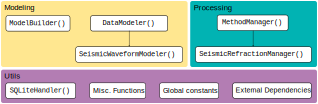
\includegraphics[width=.75\textwidth]{figures/package_structure}
	\caption{\DIFaddFL{Fundamental use case illustrating the modeling of seismic refraction data within the formikoj ecosystem.}}
	\label{fig:scheme}

\end{figure}
\DIFadd{The formikoj library provides a well thought out data management concept based on the SQLite database engine that does not require a separate server process }\footnote{\DIFadd{https://www.sqlite.org/index.html, last accessed on }\today}\DIFadd{. }\DIFaddend In particular, \DIFdelbegin \DIFdel{we present here the }\texttt{\DIFdel{SeismicWaveformModeler}} %DIFAUXCMD
\DIFdel{and }\texttt{\DIFdel{SeismicRefractionManager}} %DIFAUXCMD
\DIFdel{classes implemented within the formikoj framework, which aim at creating and processing seismic waveform data }\DIFdelend \DIFaddbegin \DIFadd{the information for each project, such as survey geometry and first break traveltimes, are stored in a SQLite database file. Using such an application file format facilitates the cross-platform design of the formikoj library, and provides fast I/O operations through concise SQL queries. The portability of the application file allows for an easy exchange of projects between partners across institutions relying on different IT infrastructures. Accordingly, the formikoj library aims at providing a transparent and customizable framework for the collaborative design of reproducible workflows. The comprehensive usage of clear error and log messages aims at supporting the user throughout the modeling and processing workflows. A meticulous exception handling ensures that the data stored in the SQLite project database is not corrupted in case of erroneous input. Moreover, documenting the user input and the respective responses of the formikoj library with the python logging module provides a timestamped command history that further enhances the transparency and repeatability of the conducted workflows.
}

\DIFadd{We present the application of the formikoj library for the modeling and processing of seismic refraction data based on the fundamental use cases presented in Figure~\ref{fig:modworkflow} and Figure~\ref{fig:procworkflow}}\DIFaddend , respectively.
\DIFdelbegin \DIFdel{Similar to RefraPy, }\DIFdelend \DIFaddbegin \begin{figure}
	\centering
	\includegraphics[width=\textwidth]{figures/workflow_modeling-crop.pdf}
	\caption{\DIFaddFL{Fundamental use case illustrating the processing of seismic refraction data within the formikoj ecosystem.}}
	\label{fig:modworkflow}
\end{figure}
\begin{figure}
	\centering
	\includegraphics[width=\textwidth]{figures/workflow_processing-crop.pdf}
	\caption{\DIFaddFL{Typical formikoj workflow for the picking of first break traveltimes from seismic waveform data.}}
	\label{fig:procworkflow}

\end{figure}
\DIFadd{These flow charts illustrate the corresponding workflows as well as the required interactions between the user, the formikoj library and third-party packages. As can be seen from Figure~\ref{fig:modworkflow} and Figure~\ref{fig:procworkflow}, the formikoj library acts as an interface between the user and more complex functionalities of third-party libraries, such as pyGIMLi for modeling and inversion of seismic refraction data.
The }\texttt{\DIFadd{SeismicWaveformModeler}} \DIFadd{and }\texttt{\DIFadd{SeismicRefractionManager}} \DIFadd{classes implement these fundamental use cases, yet their actual capabilities are continuously expanded, e.g., to address specific modeling or processing requirements as well as to enhance the user experience. To avoid redundancies in the implementation we built }\DIFaddend these classes \DIFdelbegin \DIFdel{are built }\DIFdelend upon the functionalities of existing packages such as ObsPy for the processing of seismological data \citep[][]{beyreuther2010} and pyGIMLi for the modeling and inversion of different geophysical data \citep{ruecker2017}. Other important third party dependencies refer to NumPy \citep{harris2020} and Pandas \citep{mckinney2010} for general data handling, as well as matplotlib \citep{hunter2007} and PyVista \citep{sullivan2019} for data visualization.
\DIFdelbegin \DIFdel{In the current version, we implemented and tested formikoj primarily on Linux machines , yet the library has been successfully used on all major operating systems, i.e., Linux, MacOS and Windows }\DIFdelend \DIFaddbegin 

\DIFadd{The formikoj library is primarily developed on machines running Linux Mint \num{20} or Kubuntu \num{22}.\num{04}, respectively. Testing of the library refers to carrying out the fundamental use cases for modeling and processing of seismic refraction data presented in Figure~\ref{fig:modworkflow} and \ref{fig:procworkflow}. To ensure the cross-platform applicability of the formikoj library we test these fundamental use cases also on machines running on Windows \num{10}, Windows \num{11} as well as macOS versions \num{12} and \num{13}}\DIFaddend .

\DIFdelbegin %DIFDELCMD < \begin{figure}
%DIFDELCMD < 	\centering
%DIFDELCMD < 	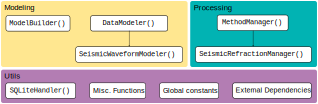
\includegraphics[width=.75\textwidth]{figures/package_structure}
%DIFDELCMD < 	%%%
%DIFDELCMD < \caption{%
{%DIFAUXCMD
\DIFdelFL{General architecture of the formikoj library comprising a utility, modeling and processing module. The base classes }\texttt{\DIFdelFL{DataModeler}} %DIFAUXCMD
\DIFdelFL{and }\texttt{\DIFdelFL{MethodManager}} %DIFAUXCMD
\DIFdelFL{can be used to build tools for specific geophysical methods, e.g., seismic refraction.}}
	%DIFAUXCMD
%DIFDELCMD < \label{fig:scheme}
%DIFDELCMD < \end{figure}
%DIFDELCMD < %%%
\DIFdelend \DIFaddbegin \subsection{\DIFadd{Generation of seismic waveform data for synthetic subsurface models}}
\DIFaddend 

\DIFdelbegin \subsection{\DIFdel{Generation of seismic waveform data for synthetic subsurface models: The }\texttt{\DIFdel{SeismicWaveformModeler}}%DIFAUXCMD
}
%DIFAUXCMD
\addtocounter{subsection}{-1}%DIFAUXCMD
%DIFDELCMD < 

%DIFDELCMD < %%%
\DIFdelend The SR method exploits the ground motion recorded by sensors installed in the surface (e.g., geophones) to characterize the propagation of seismic waves generated at well known locations (i.e., shot stations). 
The visualization of the ground motion as function of time yields a so-called seismogram for each geophone position.
Accordingly, the \texttt{SeismicWaveformModeler} class provides a flexible way to generate synthetic seismic waveform data \DIFaddbegin \DIFadd{for P-wave refraction modeling }\DIFaddend either in a python script, interactively in a jupyter notebook or an ipython shell.
To create an instance of the class the \DIFaddbegin \DIFadd{user provides the absolute or relative }\DIFaddend path to the working directory \DIFdelbegin \DIFdel{is provided }\DIFdelend as parameter to the constructor:
\DIFdelbegin %DIFDELCMD < \newline
%DIFDELCMD < \includegraphics[width=.5\textwidth]{./figures/create_swm.pdf}
%DIFDELCMD < \newline
%DIFDELCMD < \\%%%
\DIFdel{The working directoryneeds to contain a subdirectory }\textit{\DIFdel{in}}%DIFAUXCMD
\DIFdel{, whereas the output directory }\textit{\DIFdel{out}} %DIFAUXCMD
\DIFdel{will be created automatically:
}\DIFdelend \DIFaddbegin \DIFmodbegin
\begin{lstlisting}[language=Python,alsolanguage=DIFcode]
%DIF > # Import the SeismicWaveformModeler from the formikoj library
%DIF > from formikoj import SeismicWaveformModeler
%DIF > 
%DIF > # Create an instance of the SeismicWaveformModeler
%DIF > swm = SeismicWaveformModeler('.')
\end{lstlisting}
\DIFmodend
\DIFaddend 

\DIFdelbegin %DIFDELCMD < \dirtree{%
%DIFDELCMD < .1 working\_directory.
%DIFDELCMD < .2 in.
%DIFDELCMD < .2 out.
%DIFDELCMD < }
%DIFDELCMD < %%%
\DIFdelend \DIFaddbegin \begin{footnotesize}
\DIFmodbegin
\begin{DIFverbatim}[alsolanguage=DIFcode]
%DIF > INFO    : Created instance of SeismicWaveformModeler
\end{DIFverbatim}
\DIFmodend
\end{footnotesize}
\DIFaddend 

\DIFdelbegin %DIFDELCMD < \begin{table}[pos=h]
%DIFDELCMD <     %%%
%DIFDELCMD < \caption{%
{%DIFAUXCMD
\DIFdelFL{Description of the information to be provided in the columns of a measurement scheme in csv format.}}
    %DIFAUXCMD
%DIFDELCMD < \centering
%DIFDELCMD <     \begin{tabular}{clcl}
%DIFDELCMD <         \toprule
%DIFDELCMD <         %%%
\DIFdelFL{Column }%DIFDELCMD < & %%%
\textbf{\DIFdelFL{Content}} %DIFAUXCMD
%DIFDELCMD < & %%%
\textbf{\DIFdelFL{Data type}} %DIFAUXCMD
%DIFDELCMD < & %%%
\textbf{\DIFdelFL{Description}} %DIFAUXCMD
%DIFDELCMD < \\
%DIFDELCMD <         \midrule
%DIFDELCMD <         %%%
\DIFdelFL{1 }%DIFDELCMD < & %%%
\DIFdelFL{x coordinate }%DIFDELCMD < & %%%
\DIFdelFL{float }%DIFDELCMD < & %%%
\DIFdelFL{Station x coordinate, e.g., given in (m) }%DIFDELCMD < \\ 
%DIFDELCMD <         %%%
\DIFdelFL{2 }%DIFDELCMD < & %%%
\DIFdelFL{y coordinate }%DIFDELCMD < & %%%
\DIFdelFL{float }%DIFDELCMD < & %%%
\DIFdelFL{Station y coordinate, e.g., given in (m) }%DIFDELCMD < \\ 
%DIFDELCMD <         %%%
\DIFdelFL{3 }%DIFDELCMD < & %%%
\DIFdelFL{z coordinate }%DIFDELCMD < & %%%
\DIFdelFL{float }%DIFDELCMD < & %%%
\DIFdelFL{Station z coordinate, e.g., given in (m) }%DIFDELCMD < \\ 
%DIFDELCMD <         %%%
\DIFdelFL{4 }%DIFDELCMD < & %%%
\DIFdelFL{Geophone }%DIFDELCMD < & %%%
\DIFdelFL{bool }%DIFDELCMD < & %%%
\DIFdelFL{1 in case of a receiver station, 0 otherwise }%DIFDELCMD < \\ 
%DIFDELCMD <         %%%
\DIFdelFL{5 }%DIFDELCMD < & %%%
\DIFdelFL{Shot }%DIFDELCMD < & %%%
\DIFdelFL{bool }%DIFDELCMD < & %%%
\DIFdelFL{1 in case of a shot station, 0 otherwise }%DIFDELCMD < \\
%DIFDELCMD <         \bottomrule
%DIFDELCMD <     \end{tabular}
%DIFDELCMD <     \label{tab:scheme}
%DIFDELCMD < \end{table}
%DIFDELCMD < %%%
\DIFdel{The }\DIFdelend \DIFaddbegin \DIFadd{In the working directory, the }\DIFaddend required input files \DIFdelbegin \DIFdel{need to be }\DIFdelend \DIFaddbegin \DIFadd{are }\DIFaddend provided via the subdirectory \textit{in}\DIFdelbegin \DIFdel{of the working directory}\DIFdelend \DIFaddbegin \DIFadd{, whereas the modeling output will be stored in the automatically created subdirectory }\textit{\DIFadd{out}}\DIFaddend . The key input file is the measurement scheme \DIFdelbegin \DIFdel{, which }\DIFdelend \DIFaddbegin \DIFadd{as it }\DIFaddend contains information regarding the distribution of the shot and geophone stations. If provided in the unified data format\DIFaddbegin \DIFadd{, }\DIFaddend the measurement scheme is imported directly with pyGIMLi into a \texttt{DataContainer}. In case the measurement scheme is provided as a csv file\DIFaddbegin \DIFadd{, }\DIFaddend the \texttt{SeismicWaveformModeler} reads the information and writes it to a pyGIMLi \texttt{DataContainer} \DIFdelbegin \DIFdel{. In the csv format }\DIFdelend \DIFaddbegin \DIFadd{object. If provided as csv file, }\DIFaddend the measurement scheme contains a single line for each station in the survey layout, where a station either hosts a geophone or a shot, or both (see Table~\ref{tab:scheme}). The values provided in each line need to be separated by a unique delimiter, and the file must not contain a header.
\DIFaddbegin 
\begin{table}
%DIF > [pos=h]
    \caption{\DIFaddFL{Description of the information to be provided in the columns of a measurement scheme in csv format.}}
    \centering
    \begin{tabular}{clcl}
        \toprule
        \DIFaddFL{Column }& \textbf{\DIFaddFL{Content}} & \textbf{\DIFaddFL{Data type}} & \textbf{\DIFaddFL{Description}} \\
        \midrule
        \DIFaddFL{1 }& \DIFaddFL{x coordinate }& \DIFaddFL{float }& \DIFaddFL{Station x coordinate, e.g., given in (m) }\\ 
        \DIFaddFL{2 }& \DIFaddFL{y coordinate }& \DIFaddFL{float }& \DIFaddFL{Station y coordinate, e.g., given in (m) }\\ 
        \DIFaddFL{3 }& \DIFaddFL{z coordinate }& \DIFaddFL{float }& \DIFaddFL{Station z coordinate, e.g., given in (m) }\\ 
        \DIFaddFL{4 }& \DIFaddFL{Geophone }& \DIFaddFL{bool }& \DIFaddFL{1 in case of a receiver station, 0 otherwise }\\ 
        \DIFaddFL{5 }& \DIFaddFL{Shot }& \DIFaddFL{bool }& \DIFaddFL{1 in case of a shot station, 0 otherwise }\\
        \bottomrule
    \end{tabular}
    \label{tab:scheme}

\end{table}
\DIFaddend 

For the modeling of the seismic \DIFdelbegin \DIFdel{waveforms}\DIFdelend \DIFaddbegin \DIFadd{waveform data}\DIFaddend , the parameters \DIFdelbegin \DIFdel{for }\DIFdelend \DIFaddbegin \DIFadd{characterizing }\DIFaddend the base wavelet, the synthetic subsurface model and the resulting waveform datasets are provided (see Table~\ref{tab:config}) in a configuration file following the yaml format:
\DIFdelbegin %DIFDELCMD < \newline
%DIFDELCMD < 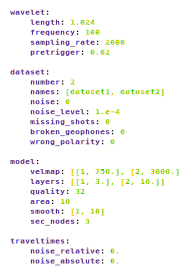
\includegraphics[width=.3\textwidth]{./figures/yaml_file.pdf}
%DIFDELCMD < \newline
%DIFDELCMD < %%%
\DIFdel{In the exemplary configurationfile shown above}\DIFdelend \DIFaddbegin 

\begin{footnotesize}
\DIFmodbegin
\begin{DIFverbatim}[alsolanguage=DIFcode]
%DIF > wavelet:
%DIF >     length: 1.024
%DIF >     frequency: 100
%DIF >     sampling_rate: 2000
%DIF >     pretrigger: 0.02
%DIF > 
%DIF > model:
%DIF >     velmap: [[1, 750], [2, 2500], [3, 4000]]
%DIF >     layers: [[1, 3], [2, 5], [3, 15]]
%DIF >     quality: 32
%DIF >     area: 10
%DIF >     smooth: [1, 10]
%DIF >     sec_nodes: 3    
%DIF > 
%DIF > dataset:
%DIF >     number: 1
%DIF >     names: [syn_data]
%DIF >     noise: 1
%DIF >     noise_level: 1e-4
%DIF >     missing_shots: 1
%DIF >     broken_geophones: 1
%DIF >     wrong_polarity: 1
%DIF >     
%DIF > traveltimes:
%DIF >     noise_relative: 0.
%DIF >     noise_absolute: 0.
\end{DIFverbatim}
\DIFmodend
\end{footnotesize}

\DIFadd{In this exemplary configuration}\DIFaddend , the first block \DIFdelbegin \DIFdel{contains information regarding the }\DIFdelend \DIFaddbegin \DIFadd{(}\texttt{\DIFadd{wavelet}}\DIFadd{) contains the parameterization of the base }\DIFaddend wavelet, which controls the modeling of the seismic waveforms \DIFdelbegin \DIFdel{as described in }\DIFdelend \DIFaddbegin \DIFadd{(see }\DIFaddend Table~\ref{tab:config}\DIFdelbegin \DIFdel{.
In the second block }\DIFdelend \DIFaddbegin \DIFadd{).
The second block (}\texttt{\DIFadd{model}}\DIFadd{) contains information regarding the synthetic subsurface model. Here, the user can define simple models with all layers considered to be parallel to the surface topography, which is inferred from the station geometry provided in the measurement scheme. The seismic velocity values for the different model regions (}\texttt{\DIFadd{velmap}}\DIFadd{) and the corresponding thickness of the different geological units (}\texttt{\DIFadd{layers}}\DIFadd{) have to be explicitly defined in the configuration file. The remaining parameters (}\texttt{\DIFadd{quality}}\DIFaddend , \DIFdelbegin \DIFdel{we }\DIFdelend \DIFaddbegin \texttt{\DIFadd{area}}\DIFadd{, }\texttt{\DIFadd{smooth}} \DIFadd{and }\texttt{\DIFadd{sec\_nodes}}\DIFadd{) refer to the properties of the mesh that is eventually used for the forward modeling of the seismic waveform data and corresponding first break traveltimes (we refer to the respective pyGIMLi resources}\footnote{\DIFadd{https://www.pygimli.org/pygimliapi/\_generated/pygimli.meshtools.html\#pygimli.meshtools.createMesh, last accessed }\today} \DIFadd{for further information).
In the third block of the exemplary configuration file (}\texttt{\DIFadd{dataset}}\DIFadd{), the user }\DIFaddend can set specific names for the datasets to be created \DIFdelbegin \DIFdel{and }\DIFdelend \DIFaddbegin \DIFadd{(}\DIFaddend the number of datasets is automatically determined\DIFdelbegin \DIFdel{. Alternatively, it is possible to }\DIFdelend \DIFaddbegin \DIFadd{), or }\DIFaddend set the number of datasets to be created and the dataset names are automatically generated with the prefix \textit{dataset\_}.
\DIFdelbegin \DIFdel{Various parameters }\DIFdelend \DIFaddbegin \DIFadd{The remaining parameters provided in the }\texttt{\DIFadd{dataset}} \DIFadd{block }\DIFaddend control the random error (\texttt{noise} \DIFdelbegin \DIFdel{) and systematic errors }\DIFdelend \DIFaddbegin \DIFadd{and }\texttt{\DIFadd{noise\_level}}\DIFadd{) as well as systematic errors (}\texttt{\DIFadd{missing\_shots}}\DIFadd{, }\texttt{\DIFadd{broken\_geophones}} \DIFadd{and }\texttt{\DIFadd{wrong\_polarity}}\DIFadd{) }\DIFaddend in the modeled seismic waveform data (see Table~\ref{tab:config} \DIFaddbegin \DIFadd{for a detailed description}\DIFaddend ).
The number and position of the shot and geophone stations affected by the systematic errors are randomly chosen with a maximum of \DIFdelbegin \DIFdel{5\% }\DIFdelend \DIFaddbegin \qty{5}{\%} \DIFaddend of the total number of stations in order to avoid a high number of invalid trace data.
The \DIFdelbegin \DIFdel{third block contains information regarding the synthetic subsurface model. For each layer the corresponding velocity (}\DIFdelend \DIFaddbegin \DIFadd{final block of the configuration file (}\DIFaddend \texttt{\DIFdelbegin \DIFdel{velmap}\DIFdelend \DIFaddbegin \DIFadd{traveltimes}\DIFaddend }) \DIFdelbegin \DIFdel{and layer thickness (}\texttt{\DIFdel{layers}}%DIFAUXCMD
\DIFdel{) need to be provided and all layers are considered to be parallel to the surface topography (geometrical information regarding the stations in the measurement scheme) . The remaining parameters, namely }\texttt{\DIFdel{quality}}%DIFAUXCMD
\DIFdel{, }\texttt{\DIFdel{area}}%DIFAUXCMD
\DIFdel{, }\texttt{\DIFdel{smooth}} %DIFAUXCMD
\DIFdelend \DIFaddbegin \DIFadd{contains data-error parameters for both the absolute error ($e_{abs}$) }\DIFaddend and \DIFdelbegin \texttt{\DIFdel{sec\_nodes}}%DIFAUXCMD
\DIFdel{, define the properties of the mesh to be used for the forward modeling (we refer to the respective pyGIMLi resources}\footnote{\DIFdel{https://www.pygimli.org/pygimliapi/\_generated/pygimli.meshtools.html\#pygimli.meshtools.createMesh, last accessed }%DIFDELCMD < \today%%%
} %DIFAUXCMD
\addtocounter{footnote}{-1}%DIFAUXCMD
\DIFdel{for further information).
Alternatively, the user can provide a more complex mesh in the binary mesh format (}\DIFdelend \DIFaddbegin \DIFadd{the relative error ($e_{rel}$) defined by the user. The data error model is then estimated as
}

\begin{equation}
	\DIFadd{\vecmat{e} = e_{abs} + \vecmat{d}\,e_{rel}\,, 
	\label{eq:esterr}
}\end{equation}
\DIFadd{where $\vecmat{d}$ denotes the forward modeled data not affected by noise, }\DIFaddend i.e., \DIFdelbegin \DIFdel{a bms file):
}%DIFDELCMD < \newline
%DIFDELCMD < \includegraphics[width=.5\textwidth]{./figures/load_mesh.pdf}
%DIFDELCMD < \newline
%DIFDELCMD < %%%
\DIFdel{The parameters in the final block control the forward modeling of the corresponding seismic traveltimes (see Table~\ref{tab:config}). A configuration file located in the input directory can be imported through the }\texttt{\DIFdel{load}} %DIFAUXCMD
\DIFdel{method:
}%DIFDELCMD < \newline
%DIFDELCMD < \includegraphics[width=.5\textwidth]{./figures/load_config.pdf}
%DIFDELCMD < \newline
%DIFDELCMD < %%%
\DIFdelend \DIFaddbegin \DIFadd{here the first break traveltimes obtained through the Dijkstra algorithm \mbox{%DIFAUXCMD
\citep{dijkstra1959}}\hskip0pt%DIFAUXCMD
. These computed error values are subsequently added to the data to obtain the noisy data as
}

\begin{equation}
	\DIFadd{\vecmat{d_{noise}}=\vecmat{d}\left(1 + \vecmat{e}\right)\,.
	\label{eq:noisydata}
}\end{equation}

\DIFaddend \begin{table*}[]
    \caption{Description of the parameters, which can be defined in a configuration file used for the modeling of the synthetic seismic data.}
    \centering
    \begin{tabular*}{\tblwidth}{@{} LCL@{}}
        \toprule
        \textbf{Parameter} & \textbf{Unit/} & \textbf{Description} \\
         & \textbf{Data type} & \\ 
        \midrule
        \textbf{\texttt{wavelet}} & & \\
         & & \\
        length & s & Length of the base wavelet, which also defines the \\
         & & length of the synthetic seismic waveform data \\ 
        frequency & Hz & Frequency of the base wavelet \\ 
        sampling\_rate & Hz & Defines temporal resolution of the seismic waveforms \\ 
        pretrigger & s & Add buffer to the seismic waveforms before the onset \\
         & & of the actual data \\
        \midrule
        \textbf{\texttt{dataset}} & & \\
         & & \\
        number & int & Number of datasets to be created \\
        names & list (string) & Names of the datasets \\
        noise & bool & 1 in case noise should be added to the synthetic \\
         & & waveforms, 0 otherwise \\
        noise\_level & - & Level of the seismic background noise \\
        missing\_shots & bool & 1 in case the datasets should be affected by missing \\
         & & shot files, 0 otherwise \\
        broken\_geophones & bool & 1 in case the datasets should comprise broken \\
         & & geophones (i.e., no data in the corresponding \\
         & & seismograms), 0 otherwise \\
        wrong\_polarity & bool & 1 in case the datasets should contain traces with \\
         & & inverse polarity, 0 otherwise \\
        \midrule
        \textbf{\texttt{model}} & & \\
         & & \\
        velmap & list & For each layer the first value defines the marker and \\
         & (float/int) & the second one the seismic velocity within the layer \\
        layers & list & For each layer the first value defines the marker and \\
         & (float/int) & the second one the thickness \\
        \midrule
        \textbf{\texttt{traveltimes}} & & \\
         & & \\
        noise\_relative & \%/100 & Relative noise to be added to the forward modeled \\
      	 & & seismic traveltimes \\
        noise\_absolute & s & Absolute noise to be added to the forward modeled \\
         & & seismic traveltimes\\
        \bottomrule
    \end{tabular*}
    \label{tab:config}
\end{table*}
\DIFdelbegin \DIFdel{Once the }\DIFdelend \DIFaddbegin 

\DIFadd{The configuration file needs to be provided via the input directory from where it can be imported through the }\texttt{\DIFadd{load}} \DIFadd{method of the }\DIFaddend \texttt{SeismicWaveformModeler}\DIFdelbegin \DIFdel{instance is parameterized the synthetic }\DIFdelend \DIFaddbegin \DIFadd{:
}\DIFmodbegin
\begin{lstlisting}[language=Python, firstnumber=6,alsolanguage=DIFcode]
%DIF > # Load and parse the configuration file
%DIF > swm.load(type='config')
\end{lstlisting}
\DIFmodend
\begin{footnotesize}
\DIFmodbegin
\begin{DIFverbatim}[alsolanguage=DIFcode]
%DIF > INFO    : Configuration loaded
\end{DIFverbatim}
\DIFmodend
\end{footnotesize}
\DIFadd{To demonstrate the ability to model }\DIFaddend seismic waveform data \DIFdelbegin \DIFdel{can be created }\DIFdelend \DIFaddbegin \DIFadd{for arbitrary subsurface conditions we do not define a simple subsurface model in the configuration file but provide a more complex model in the binary mesh format (e.g., a bms file). We prepare the model and the corresponding forward modeling mesh based on the mesh tools provided by pyGIMLi and save the mesh in the bms format (a commented version of the corresponding python script can be found in the Appendix). Similar to the configuration file, a bms file stored in the input directory can be imported into the workflow through the }\texttt{\DIFadd{load}} \DIFadd{method }\DIFaddend as follows:
\DIFdelbegin %DIFDELCMD < \newline
%DIFDELCMD < 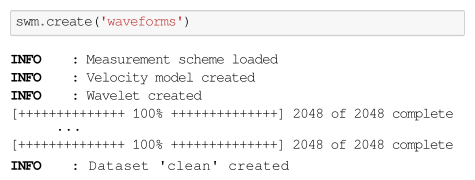
\includegraphics[width=.5\textwidth]{./figures/create_syn_data.pdf}
%DIFDELCMD < \newline
%DIFDELCMD < %%%
\DIFdel{The }\DIFdelend \DIFaddbegin \DIFmodbegin
\begin{lstlisting}[language=Python, firstnumber=8,alsolanguage=DIFcode]
%DIF > # Load the mesh into the workflow
%DIF > swm.load(type='mesh')
\end{lstlisting}
\DIFmodend
\begin{footnotesize}
\DIFmodbegin
\begin{DIFverbatim}[alsolanguage=DIFcode]
%DIF > INFO    : Mesh loaded
\end{DIFverbatim}
\DIFmodend
\end{footnotesize}
\DIFadd{The forward modeling process generating the seismic waveform data is then invoked through the }\texttt{\DIFadd{create}} \DIFadd{method:
}\DIFmodbegin
\begin{lstlisting}[language=Python, firstnumber=10,alsolanguage=DIFcode]
%DIF > # Start the modeling of the seismic waveform data
%DIF > swm.create(type='waveforms')
\end{lstlisting}
\DIFmodend
\begin{footnotesize}
\DIFmodbegin
\begin{DIFverbatim}[alsolanguage=DIFcode]
%DIF > INFO    : Measurement scheme loaded
%DIF > INFO    : Velocity model created
%DIF > INFO    : Wavelet created
%DIF > [++++++++++++++ 100% ++++++++++++++] 2048 of 2048 complete
%DIF >       ...
%DIF > [++++++++++++++ 100% ++++++++++++++] 2048 of 2048 complete
%DIF > INFO    : Dataset 'syn\_data' created
\end{DIFverbatim}
\DIFmodend
\end{footnotesize}
\DIFadd{As can be seen from the log messages, the }\DIFaddend \texttt{SeismicWaveformModeler} \DIFaddbegin \DIFadd{first }\DIFaddend loads the measurement scheme \DIFdelbegin \DIFdel{and creates the velocity model used }\DIFdelend \DIFaddbegin \DIFadd{into the workflow. In the second step, the provided mesh and the seismic velocity values defined in the configuration file are combined to create the seismic velocity model considered }\DIFaddend for the waveform modeling \DIFdelbegin \DIFdel{.
Based on the wavelet properties a Ricker wavelet is generated }\DIFdelend \DIFaddbegin \DIFadd{in this study (see Figure~\ref{fig:syndataexample}a). The model consists of a top and a bottom layer with varying thickness characterized by seismic velocity values of }\qty{750}{ms^{-1}} \DIFadd{and }\qty{4000}{ms^{-1}}\DIFadd{, respectively. In the center, the model contains an irregularly shaped anomaly associated with a seismic velocity of }\qty{2500}{ms^{-1}}\DIFadd{, i.e., the model features vertical and lateral variations in the seismic velocity distribution.
}\begin{figure}
	\centering
	\includegraphics[width=.75\textwidth]{figures/synthetic_data_example.pdf}
	\caption{\DIFaddFL{Synthetic seismic data generated with the }\texttt{\DIFaddFL{SeismicWaveformModeler}}\DIFaddFL{: }\\\DIFaddFL{(a) Two-layered subsurface model without topography characterized by a distinct anomaly in the center. Triangles along the surface indicate the positions of geophones. }\\\DIFaddFL{(b) Synthetic seismic waveform data computed from the subsurface model for a shot point (star-shaped symbol) located in the center of the profile. }\\\DIFaddFL{(c) Pseudosection illustrating the apparent velocity computed from the seismic traveltimes based on the survey geometry. }\\\DIFaddFL{(d) Subsurface model of the seismic P-wave velocity distribution obtained through the inversion of the synthetic P-wave traveltimes.}}
	\label{fig:syndataexample}

\end{figure}
\DIFadd{The third step refers to the generation of a Ricker wavelet }\DIFaddend through the pyGIMLi function \texttt{ricker} \DIFdelbegin \DIFdel{.
Subsequently, mesh}\DIFdelend \DIFaddbegin \DIFadd{as
}

\begin{equation}
	\DIFadd{u = \left(1-2\pi^2f^2t^2\right)e^{-\pi^2f^2\left(t-t_0\right)^2}\,
	\label{eq:ricker}
}\end{equation}
\DIFadd{based on the wavelet properties provided in the configuration file. In Equation~\ref{eq:ricker}, $f$ is the frequency of the wavelet given in }\unit{Hz}\DIFaddend , \DIFaddbegin \DIFadd{$t$ refers to the time base definition, i.e., the length and resolution of the wavelet in the time domain, and $t_0$ is the time offset of the wavelet.
}

\DIFadd{Based on the mesh, the }\DIFaddend velocity model and \DIFdelbegin \DIFdel{Ricker wavelet are used }\DIFdelend \DIFaddbegin \DIFadd{the Ricker wavelet we use pyGIMLi 
}\DIFaddend to solve the pressure wave equation for each shot station defined in the measurement scheme\DIFdelbegin \DIFdel{with the pyGIMLi function }\texttt{\DIFdel{solvePressureWave}}%DIFAUXCMD
\DIFdelend .
The resultant \DIFdelbegin \DIFdel{waveforms }\DIFdelend \DIFaddbegin \DIFadd{seismograms are extracted }\DIFaddend at the corresponding geophone stations\DIFdelbegin \DIFdel{are extracted and stored }\DIFdelend \DIFaddbegin \DIFadd{, gathered for each shot position }\DIFaddend in an ObsPy \texttt{Stream} \DIFdelbegin \DIFdel{data structure.
}%DIFDELCMD < \clearpage
%DIFDELCMD < %%%
\DIFdel{A directory for each dataset defined in the configuration file will be created in the }\DIFdelend \DIFaddbegin \DIFadd{object and saved in the }\DIFaddend output directory (\textit{out}) \DIFdelbegin \DIFdel{:
}%DIFDELCMD < 

%DIFDELCMD < \dirtree{%
%DIFDELCMD < .1 working\_directory.
%DIFDELCMD < .2 in.
%DIFDELCMD < .2 out.
%DIFDELCMD < .3 dataset1.
%DIFDELCMD < .4 data.
%DIFDELCMD < .5 protocol.txt.
%DIFDELCMD < .5 station\_coords.csv.
%DIFDELCMD < .5 Shot\_1001.syn.
%DIFDELCMD < .5 ....
%DIFDELCMD < .5 Shot\_10nn.syn.
%DIFDELCMD < .4 dataset1\_tt.pck.
%DIFDELCMD < .4 info.txt.
%DIFDELCMD < }
%DIFDELCMD < %%%
\DIFdel{In }\DIFdelend \DIFaddbegin \DIFadd{as shown here:
}\dirtree{%
.1 working\_directory.
.2 in.
.2 out.
.3 syn\_data.
.4 data.
.5 protocol.txt.
.5 station\_coords.csv.
.5 Shot\_1001.syn.
.5 ....
.5 Shot\_10nn.syn.
.4 syn\_data\_tt.pck.
.4 info.txt.
}
\DIFadd{In particular, }\DIFaddend the subdirectory \textit{data} \DIFdelbegin \DIFdel{, the synthetic seismic waveforms are stored in a separate shot file for each shot position }\DIFdelend \DIFaddbegin \DIFadd{contains a separate file }\DIFaddend in the miniseed format \citep{ahern2012, ringler2015} \DIFdelbegin \DIFdel{with }\DIFdelend \DIFaddbegin \DIFadd{for each shot position, where }\DIFaddend the file extension \textit{syn} \DIFdelbegin \DIFdel{to identify the forward modeled shot files , e. 
g., Shot\_1001.syn.
}\DIFdelend \DIFaddbegin \DIFadd{indicates that the shot files contain forward modeled seismic waveform data. 
}\DIFaddend The measurement protocol (protocol.txt) and the station coordinates provided as a csv file (station\_coords.csv) are also stored in this directory. The header of the measurement protocol contains the survey parameters\DIFdelbegin \DIFdel{required for the processing of the seismic waveforms, namely }\DIFdelend \DIFaddbegin \DIFadd{, e.g., }\DIFaddend sampling rate, recording length, number of geophones and geophone spacing. Moreover, the protocol associates each shot file of the dataset \DIFdelbegin \DIFdel{to }\DIFdelend \DIFaddbegin \DIFadd{with }\DIFaddend a specific location \DIFdelbegin \DIFdel{within }\DIFdelend \DIFaddbegin \DIFadd{in }\DIFaddend the survey geometry \DIFdelbegin \DIFdel{, i.e., }\DIFdelend with respect to the geophone positions\DIFdelbegin \DIFdel{:
}%DIFDELCMD < \newline
%DIFDELCMD < \includegraphics[width=.3\textwidth]{./figures/protocol.pdf}
%DIFDELCMD < \newline
%DIFDELCMD < %%%
\DIFdelend \DIFaddbegin \DIFadd{, e.g.:
}\begin{footnotesize}
\DIFmodbegin
\begin{DIFverbatim}[alsolanguage=DIFcode]
%DIF >  #############################
%DIF >    Line: SYN_syn_data             
%DIF >    Sampling rate: 2000 Hz    
%DIF >    Recording length: 0.512 s 
%DIF >    Number of geophones: 48   
%DIF >    Geophone spacing: 2 m     
%DIF >  #############################
%DIF >  
%DIF >      File number | Station
%DIF >          1001    |   G001
%DIF >            :     |     :
%DIF >          1048    |   G048
\end{DIFverbatim}
\DIFmodend
\end{footnotesize}
\DIFaddend The auxiliary file info.txt \DIFdelbegin \DIFdel{provided in }\DIFdelend \DIFaddbegin \DIFadd{exported to }\DIFaddend the dataset directory summarizes the parameters from the configuration file \DIFdelbegin \DIFdel{and }\DIFdelend \DIFaddbegin \DIFadd{as well as }\DIFaddend information regarding the simulated systematic errors in the synthetic seismic waveform data\DIFdelbegin \DIFdel{:
}%DIFDELCMD < \newline
%DIFDELCMD < 
\includegraphics[width=.3\textwidth]{./figures/info.pdf}
%DIFDELCMD < \newline
%DIFDELCMD < %%%
\DIFdel{Synthetic traveltimes (}\texttt{\DIFdel{swm.create('traveltimes')}}%DIFAUXCMD
\DIFdel{) are stored in the dataset directory as udf files, }\DIFdelend \DIFaddbegin \DIFadd{, e.g.:
}\begin{footnotesize}
\DIFmodbegin
\begin{DIFverbatim}[alsolanguage=DIFcode]
%DIF > Number of geophones: 48
%DIF > Number of shots: 48
%DIF > Recording length (s): 0.512
%DIF > Sampling frequency (Hz): 2000
%DIF > Wavelet type: Ricker
%DIF > Frequency of the wavelet (Hz): 100
%DIF > 
%DIF > Missing shot(s): 11
%DIF > Broken geophone(s): 13
%DIF > Wrong polarity geophone(s): 26
\end{DIFverbatim}
\DIFmodend
\end{footnotesize}

\DIFadd{Figure~\ref{fig:syndataexample}b presents the seismic waveform data forward modeled for a shot point located in the center of the profile. The seismograms are shown as curves, whereas the strength of the amplitudes is added as color-coded information. In the seismograms we see clear first onsets along the entire profile, yet receivers 3 and 45 were modeled as broken geophones, i.e., the corresponding seismograms contain solely noise. Crosses overlaid on the valid seismograms at the respective first onset indicate the first break traveltimes $tt$ between the shot and the receiver. In addition to the missing first break traveltimes for the broken receivers, we manually added a systematic error, i.e., we set an erroneous traveltime for receiver 36, to demonstrate how such outliers can be identified in a so-called pseudosection.
}

\DIFadd{Pseudosections are a useful tool for the analysis of the data quality by presenting the data based on the positions of shots and receivers. Such a visualization allows for the detection of outliers and their spatial distribution as necessary to understand possible sources of error. In case of the SRT, a pseudosection as presented in Figure~\ref{fig:syndataexample}c, illustrates apparent velocity ($v_{app}$) values computed as
}

\begin{equation}
	\DIFadd{v_{app}=\frac{aoffset}{tt}\,,
	\label{eq:vapp}
}\end{equation}
\DIFadd{where $aoffset$ refers to the absolute offset between shot and receiver. The $v_{app}$ values are plotted at pseudolocations, where the location along profile direction is defined by the midpoint of the corresponding shot-receiver pair and the pseudodepth is computed as $1/3$ of $aoffset$.
As demonstrated in Figure~\ref{fig:syndataexample}c, a pseudosection allows for the identification of missing data (}\DIFaddend e.g., \DIFdelbegin \DIFdel{dataset1\_tt.pck.The file extension }\textit{\DIFdel{pck}} %DIFAUXCMD
\DIFdel{is an abbreviation of the word 'pick' and }\DIFdelend \DIFaddbegin \DIFadd{receiver 3 and 45) as well as systematic errors or outliers, i.e., velocities erroneously influenced by a single shot or receiver (see receiver 36). The main assumption here is that the pseudosection should reveal smooth transitions between lateral and vertical neighbors, considering that the data were collected with gradual changes in the position of the source (i.e., hammer blow) and the receiver (i.e., geophone). The pseudosection will reveal large variations in case of abrupt changes in the topography or the geometry of the array, yet this can be taken into account by the user during the identification of outliers and possible systematic errors.
}

\DIFadd{Based on pseudosections erroneous traveltimes can be identified and subsequently removed or corrected, which is a critical processing step prior to the inversion of the data. The inversion of first break traveltimes aims at resolving a model of the P-wave velocity of the subsurface materials, where systematic errors in the data would lead to the creation of artifacts in the imaging results or hinder the convergence of the inversion.
Considering the multitude of available inversion frameworks we do not include a new inversion strategy in the formikoj library. Instead the processed data can be exported in any format required for the use of commercial inversion algorithms, or can be linked directly to other open-source libraries. In our case, we refer to the modeling and inversion capabilities of pyGIMLi \mbox{%DIFAUXCMD
\citep{ruecker2017}}\hskip0pt%DIFAUXCMD
.
pyGIMLi uses a generalized Gauss-Newton method to solve the inversion problem through the minimization of an objective function given as:
}

\begin{equation}
	\DIFadd{\parallel\vecmat{W}_d\left(\mathcal{F}\left(\vecmat{m}\right)-\vecmat{d}\right)\parallel_2^2+\lambda\parallel\vecmat{W}_m\left(\vecmat{m}-\vecmat{m}_0\right)\parallel_2^2\rightarrow\textrm{min}
	\label{eq:objfct}
}\end{equation}
\DIFadd{The first term on the right-hand side of Equation~\ref{eq:objfct} }\DIFaddend refers to the \DIFaddbegin \DIFadd{data misfit. $\vecmat{W}_d$ is the data weighting matrix holding the reciprocals of the data errors, $\vecmat{d}$ denotes the data vector holding the input data (}\DIFaddend first break traveltimes\DIFdelbegin \DIFdel{saved in the file.}\DIFdelend \DIFaddbegin \DIFadd{), $\vecmat{m}$ is the model vector representing the target parameter (seismic P-wave velocity values), and $\mathcal{F}\left(\vecmat{m}\right)$ is the model response.
The second term denotes represents the regularization, where $\vecmat{W}_m$ and $\vecmat{m}_0$ are the model constraint matrix and the reference model, respectively. The regularization parameter $\lambda$ balances the influence of the data misfit and the regularization term on the inversion process.
}\DIFaddend 

\DIFaddbegin \DIFadd{The inversion of the synthetic first break traveltimes considered here resolves the subsurface model presented in Figure~\ref{fig:syndataexample}d, which is given in terms of the spatial variations of the seismic P-wave velocity, i.e., reflecting the associated lateral and vertical variations. Depending on the survey geometry the inversion can resolve subsurface models in both 2D or 3D. 
To aid in the evaluation of this inversion result we superimposed the known interfaces between the different subsurface unit of the synthetic model. As can be seen from this plot, the imaging result resolves the fundamental structural features  and reflects the P-wave velocity distribution of the synthetic subsurface model. Deviations from the true velocity model are due to the smoothness-constraint inversion scheme applied by pyGIMLi. To obtain sharper contrasts between the different subsurface units in the imaging result structural constraints could be incorporated in the inversion, e.g., as demonstrated by \mbox{%DIFAUXCMD
\citep{steiner2021}}\hskip0pt%DIFAUXCMD
; yet, the exploration of different inversion strategies is beyond the scope of this study. We consider Figure~\ref{fig:syndataexample} to demonstrate the applicability of the }\texttt{\DIFadd{SeismicWaveformModeler}} \DIFadd{class for generating synthetic seismic waveform data to be used in numerical P-wave refraction seismic investigations.
}

\DIFaddend \subsection{Processing of seismic refraction datasets\DIFdelbegin \DIFdel{: the }\texttt{\DIFdel{SeismicRefractionManager}}%DIFAUXCMD
\DIFdelend }

The \DIFdelbegin \DIFdel{SR }\DIFdelend \DIFaddbegin \DIFadd{seismic refraction (SR) }\DIFaddend method is based on the measurement of the traveltimes of seismic waves determined from the the first onset of the seismic energy recorded by geophones. In the SRT, the inversion of traveltimes gathered from tens to hundreds of seismograms permits the computation of variations in the seismic velocities in an imaging framework. Measuring the traveltimes in seismograms (i.e., first break picking) is commonly done manually (or semi-automatically) in an iterative process. The signal-to-noise ratio in the recorded seismograms substantially influences the quality of the traveltimes picked in the seismograms, and thus \DIFaddbegin \DIFadd{the seismic velocity model obtained through the inversion. Accordingly, }\DIFaddend a proper enhancement of the perceptibility of the first onsets is crucial.

\DIFdelbegin \DIFdel{Accordingly, the }\DIFdelend \DIFaddbegin \DIFadd{The }\DIFaddend \texttt{SeismicRefractionManager} class provides functionalities that permit the processing of seismic waveform data for a refraction seismic analysis. These functionalities involve the reading of seismic waveform data, combining the data with information about the survey geometry, processing of the waveforms as well as the picking of first break traveltimes. Since the first break picking is a highly interactive process, the \texttt{SeismicRefractionManager} is designed primarily for usage from within an ipython shell. \DIFaddbegin \DIFadd{The first break traveltimes determined with the}\\ \texttt{\DIFadd{SeismicRefractionManager}} \DIFadd{represent the input data, e.g., for the }\texttt{\DIFadd{TravelTimeManager}} \DIFadd{of pyGIMLi \mbox{%DIFAUXCMD
\citep{ruecker2017}}\hskip0pt%DIFAUXCMD
. This is particularly relevant as the }\texttt{\DIFadd{TravelTimeManager}} \DIFadd{provides an inversion framework for first break traveltimes, yet not a framework for the processing of seismic waveform data.
For the demonstration of the fundamental }\texttt{\DIFadd{SeismicRefractionManager}} \DIFadd{capabilities we consider the synthetic seismic data created with the}\\ \texttt{\DIFadd{SeismicWaveformModeler}} \DIFadd{above, which illustrates that both classes can be combined in subsequent workflows. 
}\DIFaddend 

\subsubsection{Compiling the survey information and creating a project}

\DIFdelbegin \DIFdel{An instance of the}\texttt{\DIFdel{SeismicRefractionManager}} %DIFAUXCMD
\DIFdel{can be created by providing the path to the working directory as parameter to the constructor.
Based on the content of the working directory, the }\texttt{\DIFdel{SeismicRefractionManager}} %DIFAUXCMD
\DIFdel{automatically decides whether (i) to start in the data preview mode, (ii) }\DIFdelend \DIFaddbegin \DIFadd{To }\DIFaddend create a new \DIFdelbegin \DIFdel{project, or (iii) }\DIFdelend \DIFaddbegin \DIFadd{or }\DIFaddend load an existing \DIFdelbegin \DIFdel{project from disk.
}%DIFDELCMD < 

%DIFDELCMD < %%%
\DIFdel{The data preview mode is primarily initiated if the provided working directory contains seismic shot files:
}%DIFDELCMD < \newline
%DIFDELCMD < \includegraphics[width=.5\textwidth]{./figures/data_preview_mode.pdf}
%DIFDELCMD < \newline
%DIFDELCMD < %%%
\DIFdel{To create or load a project}\DIFdelend \DIFaddbegin \texttt{\DIFadd{SeismicRefractionManager}} \DIFadd{project}\DIFaddend , the working directory needs to contain specific subdirectories:

\dirtree{%
.1 working\_directory.
.2 01\_data.
.3 raw.
.2 02\_geom.
.2 03\_proc.
}
In this directory structure, the seismic shot files are stored in \textit{01\_data/raw} and the geometry file (\textit{geometry.csv}) is provided in \textit{02\_geom}.
\DIFdelbegin %DIFDELCMD < 

%DIFDELCMD < %%%
\DIFdelend The geometry file is a csv file that provides an abstract representation of the survey layout and must not contain a header. The fundamental element for the description of the survey layout is the station, which refers either to a geophone position, a shot position or a position with co-located shot and geophone. For each station the geometric and semantic information described in Table~\ref{tab:geometry} are provided column-wise, i.e., each line in the geometry file corresponds to a single station with a unique position within the survey layout. 
\begin{table}
[pos=h]
    \caption{Description of the information to be provided in the columns of the geometry file.}
    \centering
    \begin{tabular}{clcl}
        \toprule
        \DIFdelbeginFL \DIFdelFL{Col }\DIFdelendFL \DIFaddbeginFL \textbf{\DIFaddFL{Col}} \DIFaddendFL & \textbf{Content} & \textbf{Data type} & \textbf{Description} \\
        \midrule
        1 & x coordinate & float & Station x coordinate, e.g., given in (m) \\ 
        2 & y coordinate & float & Station y coordinate, e.g., given in (m) \\ 
        3 & z coordinate & float & Station z coordinate, e.g., given in (m) \\ 
        4 & Geophone & bool & 1 if a geophone was deployed at station, 0 otherwise \\ 
        5 & Shot & int & The numerical part of the file name, e.g., 1001, if a shot was conducted \\
          & & & at this station, -1 otherwise \\ 
        6 & First geophone & int & First active geophone (-1 if no shot was conducted at the station) \\ 
        7 & Number of geophones & int & Number of active geophones (-1 if no shot was conducted at the station) \\
        \bottomrule
    \end{tabular}
    \label{tab:geometry}
\end{table}
\DIFaddbegin \DIFadd{For the synthetic dataset considered in this study, the 2D station coordinates are provided in the geometry file, whereas the z coordinate is assumed to be }\qty{0}{m} \DIFadd{along the entire profile, as illustrated in Table~\ref{tab:syn_geometry}; thus, reflecting the lack of surface topography in the synthetic model (see Figure~\ref{fig:syndataexample}a). In the column }\textbf{\DIFadd{Geo}} \DIFadd{the geometry file contains the value 1 (True) for each station except the station located at }\qty{24}{m} \DIFadd{referring to the broken geophone modeled by the }\texttt{\DIFadd{SeismicWaveformModeler}}\DIFadd{. When compiling the geometry file we also need to take into account the missing shot at station 11, i.e., the station located at }\qty{20}{m} \DIFadd{along profile direction, and set the corresponding value to \num{-1}. 
The column }\textbf{\DIFadd{1st Geo}} \DIFadd{indicates the first active geophone along the profile for each shot file, which for the synthetic dataset considered here is the geophone deployed at the first station along the entire profile. In particular, the column }\textbf{\DIFadd{1st Geo}} \DIFadd{allows the reproduction of roll-along survey geometries, where in the first segment the first active geophone is always the geophone at station 1. Considering 48 geophones deployed in each segment, and an overlap of }\qty{50}{\%}\DIFadd{, the first geophone for the consecutive segments would be 25, 49, 73, 97, and so on. 
}\begin{table}
   \caption{\DIFaddFL{Excerpt from the geometry file describing the survey geometry of the synthetic dataset generated in this study.}}
    \centering
    \begin{tabular}{rrrcrrr}
        \toprule
        \textbf{\DIFaddFL{x (m)}} & \textbf{\DIFaddFL{y (m)}} & \textbf{\DIFaddFL{z (m)}} & \textbf{\DIFaddFL{Geo}} & \textbf{\DIFaddFL{Shot}} & \textbf{\DIFaddFL{1st Geo}} & \textbf{\DIFaddFL{\# Geo}} \\
        \midrule
		\DIFaddFL{0.0 }& \DIFaddFL{0.0 }& \DIFaddFL{0.0 }& \DIFaddFL{1 }& \DIFaddFL{1001 }& \DIFaddFL{1 }& \DIFaddFL{48 }\\
		\DIFaddFL{2.0 }& \DIFaddFL{0.0 }& \DIFaddFL{0.0 }& \DIFaddFL{1 }& \DIFaddFL{1002 }& \DIFaddFL{1 }& \DIFaddFL{48 }\\
        \DIFaddFL{\vdots }& \DIFaddFL{\vdots }& \DIFaddFL{\vdots }& \DIFaddFL{\vdots }& \DIFaddFL{\vdots }& \DIFaddFL{\vdots }& \DIFaddFL{\vdots }\\
		\DIFaddFL{20.0 }& \DIFaddFL{0.0 }& \DIFaddFL{0.0 }& \DIFaddFL{1 }& \DIFaddFL{-1 }& \DIFaddFL{1 }& \DIFaddFL{48 }\\
        \DIFaddFL{\vdots }& \DIFaddFL{\vdots }& \DIFaddFL{\vdots }& \DIFaddFL{\vdots }& \DIFaddFL{\vdots }& \DIFaddFL{\vdots }& \DIFaddFL{\vdots }\\
        \DIFaddFL{24.0 }& \DIFaddFL{0.0 }& \DIFaddFL{0.0 }& \DIFaddFL{0 }& \DIFaddFL{1013 }& \DIFaddFL{1 }& \DIFaddFL{48 }\\
        \DIFaddFL{\vdots }& \DIFaddFL{\vdots }& \DIFaddFL{\vdots }& \DIFaddFL{\vdots }& \DIFaddFL{\vdots }& \DIFaddFL{\vdots }& \DIFaddFL{\vdots }\\
		\DIFaddFL{92.0 }& \DIFaddFL{0.0 }& \DIFaddFL{0.0 }& \DIFaddFL{1 }& \DIFaddFL{1047 }& \DIFaddFL{1 }& \DIFaddFL{48 }\\
		\DIFaddFL{94.0 }& \DIFaddFL{0.0 }& \DIFaddFL{0.0 }& \DIFaddFL{1 }& \DIFaddFL{1048 }& \DIFaddFL{1 }& \DIFaddFL{48 }\\
        \bottomrule
    \end{tabular}
    \label{tab:syn_geometry}

\end{table}
\DIFaddend 

\DIFaddbegin \DIFadd{An instance of the }\texttt{\DIFadd{SeismicRefractionManager}} \DIFadd{can be created by providing the path to the working directory as parameter to the constructor. Depending on the content of the working directory, the }\texttt{\DIFadd{SeismicRefractionManager}} \DIFadd{automatically decides whether (i) to start in the data preview mode (first break picking not possible), (ii) create a new project, or (iii) load an existing project from disk.
}\DIFaddend In case the shot files as well as the geometry file are provided and a basic sanity check of the geometry file was successful, the \texttt{SeismicRefractionManager} creates a new project:
\DIFdelbegin %DIFDELCMD < \newline
%DIFDELCMD < \includegraphics[width=.5\textwidth]{./figures/create_project.pdf}
%DIFDELCMD < \newline
%DIFDELCMD < %%%
\DIFdel{In particular}\DIFdelend \DIFaddbegin \DIFmodbegin
\begin{lstlisting}[language=Python, firstnumber=1,alsolanguage=DIFcode]
%DIF > # Import the SeismicRefractionManager from the formikoj library
%DIF > from formikoj import SeismicRefractionManager
%DIF > 
%DIF > # Create an instance of the SeismicRefractionManager
%DIF > srm = SeismicRefractionManager('.')
\end{lstlisting}
\DIFmodend
\begin{footnotesize}
\DIFmodbegin
\begin{DIFverbatim}[alsolanguage=DIFcode]
%DIF > INFO    : Read geometry information from file
%DIF > INFO    : Extracted shot geometry
%DIF > INFO    : Extracted receiver geometry
%DIF > INFO    : Applied geometry
%DIF > INFO    : Standard pickset 'picks' created
%DIF > INFO    : Pickset 'picks' loaded
%DIF > INFO    : 'picks' set as active pickset
%DIF > Progress <==============================> 100.0% completed
%DIF > INFO    : Read 48 files
\end{DIFverbatim}
\DIFmodend
\end{footnotesize}
\DIFadd{In a first step}\DIFaddend , the \texttt{SeismicRefractionManager} creates an SQLite database \DIFdelbegin \DIFdel{(prj.db }\DIFdelend \DIFaddbegin \textit{\DIFadd{prj.db}} \DIFaddend in the working directory \DIFdelbegin \DIFdel{) to store the geometry information, whereby the stations are consecutively numbered }\DIFdelend \DIFaddbegin \DIFadd{based on the entity-relationship diagram shown in Figure~\ref{fig:database}.
}\begin{figure}
	\centering
	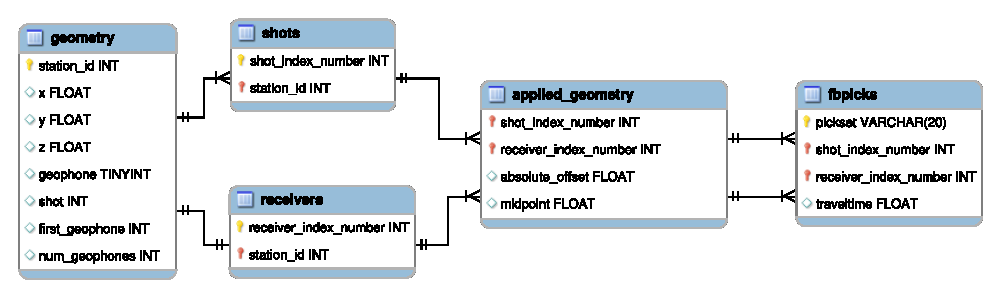
\includegraphics[width=.75\textwidth]{figures/srm_erd.eps}
	\caption{\DIFaddFL{Entity-relationship diagram illustrating the SQLite database used in a }\texttt{\DIFaddFL{SeismicRefractionManager}} \DIFaddFL{project to store an manage processing related information.}}
	\label{fig:database}

\end{figure}
\DIFadd{The geometry information is then read from the geometry file and stored in the database table }\textit{\DIFadd{geometry}} \DIFadd{with consecutively numbered stations }\DIFaddend (see Figure~\ref{fig:statnum}). To allow for an efficient data selection \DIFdelbegin \DIFdel{through }\DIFdelend \DIFaddbegin \DIFadd{for }\DIFaddend the user the \texttt{SeismicRefractionManager} \DIFdelbegin \DIFdel{links }\DIFdelend \DIFaddbegin \DIFadd{creates database tables }\textit{\DIFadd{shots}} \DIFadd{an d}\textit{\DIFadd{receivers}}\DIFadd{, which link }\DIFaddend the station numbers to shot index numbers (SIN) and receiver index numbers (RIN)\DIFdelbegin \DIFdel{assigned to shot and receiver stations, respectively(see Figure~\ref{fig:statnum}). Based on this information, the geometry is applied}\DIFdelend , \DIFaddbegin \DIFadd{respectively. For each shot-receiver pair the corresponding SIN and RIN are stored in the table }\textit{\DIFadd{applied\_geometry}} \DIFadd{together with the absolute offset and midpoint between these stations, }\DIFaddend i.e., the \DIFdelbegin \DIFdel{database tables required for the processing of the seismic waveform data are created.
In particular, }\DIFdelend \DIFaddbegin \DIFadd{geometry is applied.
In the last step, the database table }\textit{\DIFadd{fbpicks}} \DIFadd{is created, which stores }\DIFaddend the first break traveltimes for each SIN-RIN pair \DIFdelbegin \DIFdel{are stored in a dedicated database table }\textit{\DIFdel{fbpicks}} %DIFAUXCMD
\DIFdelend together with the name of the corresponding pickset, i.e., \DIFdelbegin \DIFdel{the }\DIFdelend a common label for an entire set of first break traveltimes. By default, each project contains the default pickset 'picks', which is loaded and activated on startup. Once the database is initialized, the waveform data are read from disk and the project is ready for processing.
\begin{figure}
	\centering
	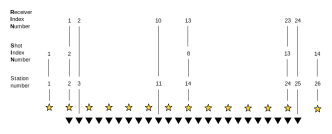
\includegraphics[width=.75\textwidth]{figures/station_numbering.pdf}
	\caption{The \texttt{SeismicRefractionManager} addresses the stations through consecutive station numbers based on the sort order in the geometry file. The shot index numbers (SIN) and receiver index numbers (RIN) are assigned to the shot and receiver stations separately to allow for an intuitive data handling for the user.}
	\label{fig:statnum}

\end{figure}

\DIFdelbegin \DIFdel{If a database file is already present in the working directory, the project information, the seismic waveforms as well as the default pickset 'picks' are automatically loaded:
}%DIFDELCMD < \newline
%DIFDELCMD < \includegraphics[width=.5\textwidth]{./figures/load_project.pdf}
%DIFDELCMD < 

%DIFDELCMD < %%%
\DIFdel{For a project with a successfully applied geometry , }\DIFdelend \DIFaddbegin \subsubsection{\DIFadd{Selecting and visualizing seismic waveform data}}
\DIFadd{Once the geometry is applied }\DIFaddend the \texttt{select} method of the \texttt{SeismicRefractionManager} allows to gather the seismic \DIFdelbegin \DIFdel{waveforms }\DIFdelend \DIFaddbegin \DIFadd{waveform data }\DIFaddend based on a common \DIFdelbegin \DIFdel{shot (}\DIFdelend \DIFaddbegin \DIFadd{absolute offset (}\DIFaddend \texttt{\DIFdelbegin \DIFdel{sin}\DIFdelend \DIFaddbegin \DIFadd{aoffset}\DIFaddend }), a common \DIFdelbegin \DIFdel{receiver }\DIFdelend \DIFaddbegin \DIFadd{RIN }\DIFaddend (\texttt{rin})\DIFdelbegin \DIFdel{or the common absolute offset (}\DIFdelend \DIFaddbegin \DIFadd{, or a common SIN (}\DIFaddend \texttt{\DIFdelbegin \DIFdel{aoffset}\DIFdelend \DIFaddbegin \DIFadd{sin}\DIFaddend })
\DIFdelbegin \DIFdel{:
}%DIFDELCMD < \newline
%DIFDELCMD < \includegraphics[width=.5\textwidth]{./figures/select.pdf}
%DIFDELCMD < %%%
\DIFdelend \DIFaddbegin \DIFmodbegin
\begin{lstlisting}[language=Python, firstnumber=6,alsolanguage=DIFcode]
%DIF > # Select traces with common absolute offset
%DIF > srm.select(by='aoffset', num=6)
\end{lstlisting}
\DIFmodend
\begin{footnotesize}
\DIFmodbegin
\begin{DIFverbatim}[alsolanguage=DIFcode]
%DIF > INFO    : 88 traces selected
\end{DIFverbatim}
\DIFmodend
\end{footnotesize}
\DIFmodbegin
\begin{lstlisting}[language=Python, firstnumber=8,alsolanguage=DIFcode]
%DIF > # Select traces with receiver
%DIF > srm.select(by='rin', num=10)
\end{lstlisting}
\DIFmodend
\begin{footnotesize}
\DIFmodbegin
\begin{DIFverbatim}[alsolanguage=DIFcode]
%DIF > INFO    : 48 traces selected
\end{DIFverbatim}
\DIFmodend
\end{footnotesize}
\DIFmodbegin
\begin{lstlisting}[language=Python, firstnumber=10,alsolanguage=DIFcode]
%DIF > # Select traces with receiver
%DIF > srm.select(by='sin', num=23)
\end{lstlisting}
\DIFmodend
\begin{footnotesize}
\DIFmodbegin
\begin{DIFverbatim}[alsolanguage=DIFcode]
%DIF > INFO    : 48 traces selected
\end{DIFverbatim}
\DIFmodend
\end{footnotesize}
\DIFaddend 

\DIFdelbegin \subsubsection{\DIFdel{Visualization and enhancement of the seismic waveform data}}
%DIFAUXCMD
\addtocounter{subsubsection}{-1}%DIFAUXCMD
\DIFdel{Calling the }\DIFdelend \DIFaddbegin \DIFadd{Figure~\ref{fig:spectrum} shows the frequency spectrum of the currently selected traces, which can be computed and visualized through the }\DIFaddend \texttt{plot} method\DIFdelbegin \DIFdel{without passing any parameter allows for the visualization of the }\DIFdelend \DIFaddbegin \DIFadd{:
}\DIFmodbegin
\begin{lstlisting}[language=Python, firstnumber=12,alsolanguage=DIFcode]
%DIF > # Plot the frequency spectrum
%DIF > srm.plot(type='spectrum')
\end{lstlisting}
\DIFmodend
\DIFadd{The }\texttt{\DIFadd{SeismicRefractionManager}} \DIFadd{resolves the frequency spectrum by computing the stacking the power spectral density ($psd$) of the seismograms $s\left(t\right)$ as
}

\begin{equation}
	\DIFadd{psd=10\log_{10}\left(\frac{\lvert \textrm{fft}\left(s\left(t\right)\right)\rvert^2}{N}\right)\,,
}\end{equation}
\DIFadd{where $\textrm{fft}$ refers to the fast fourier transformation (FFT) and $N$ is the number of the considered seismograms.
The frequency spectrum provides information regarding the amplitudes associated to different frequencies in the seismograms, which can be use for the identification of the dominating frequencies as required for the selection and application of adequate filters such as lowpass, highpass, bandpass and bandstop implemented in ObsPy \mbox{%DIFAUXCMD
\citep{beyreuther2010}}\hskip0pt%DIFAUXCMD
.
To enhance the signal-to-noise ratio of the seismograms the user can apply the respective filters through the }\texttt{\DIFadd{filter}} \DIFadd{method, which utilizes the frequency filters implemented in the ObsPy package \mbox{%DIFAUXCMD
\citep[lowpass, highpass, bandpass and bandstop;][]{beyreuther2010}}\hskip0pt%DIFAUXCMD
, e.g.:
}\DIFmodbegin
\begin{lstlisting}[language=Python, firstnumber=14,alsolanguage=DIFcode]
%DIF > # Apply bandpass filter
%DIF > srm.filter(type='bandpass', freqmin=10, freqmax=120)
\end{lstlisting}
\DIFmodend
\begin{footnotesize}
\DIFmodbegin
\begin{DIFverbatim}[alsolanguage=DIFcode]
%DIF > INFO    : Applied bandpass filter (10.0 to 120.0 Hz)
\end{DIFverbatim}
\DIFmodend
\end{footnotesize}
\begin{figure}
	\centering
	\includegraphics[width=.75\textwidth]{figures/spectrum.pdf}
	\caption{\DIFaddFL{The frequency spectrum illustrates the frequency content of the currently selected traces, which allows for the identification of frequency ranges associated to noise allowing for the definition of corresponding frequency filter settings.}}
	\label{fig:spectrum}

\end{figure}
\DIFadd{In this example, the filter is solely applied to the }\DIFaddend currently selected traces\DIFdelbegin \DIFdel{:
}%DIFDELCMD < \newline
%DIFDELCMD < \includegraphics[width=.5\textwidth]{./figures/plot.pdf}
%DIFDELCMD < \newline
%DIFDELCMD < %%%
\DIFdel{Once opened}\DIFdelend \DIFaddbegin \DIFadd{, yet setting the parameter }\texttt{\DIFadd{onhold}} \DIFadd{as }\texttt{\DIFadd{True}} \DIFadd{automatically filters all subsequently selected traces with the same filter settings, e.g.:
}\DIFmodbegin
\begin{lstlisting}[language=Python, firstnumber=16,alsolanguage=DIFcode]
%DIF > # Apply lowpass filter
%DIF > srm.filter(type='lowpass', freq=200, onhold=True)
\end{lstlisting}
\DIFmodend
\begin{footnotesize}
\DIFmodbegin
\begin{DIFverbatim}[alsolanguage=DIFcode]
%DIF > INFO    : Applied 200.0 Hz lowpass filter
%DIF > INFO    : Set filter hold on
\end{DIFverbatim}
\DIFmodend
\end{footnotesize}

\DIFadd{The currently selected traces can be visualized by calling the }\texttt{\DIFadd{plot}} \DIFadd{method without passing any parameter:
}\DIFmodbegin
\begin{lstlisting}[language=Python, firstnumber=18,alsolanguage=DIFcode]
%DIF > # Plot selected traces
%DIF > srm.plot()
\end{lstlisting}
\DIFmodend
\DIFadd{By default}\DIFaddend , the seismogram plot visualizes the seismic waveforms in a combination of wiggle trace and variable area mode, i.e., the trace data are shown as curves. The area of the curves is colored red for negative and blue for positive amplitudes, respectively (not shown for brevity). Pressing the up or down arrow key on the keyboard toggles \DIFdelbegin \DIFdel{the visualization mode }\DIFdelend between variable area and variable density \DIFdelbegin \DIFdel{. In variable density modethe }\DIFdelend \DIFaddbegin \DIFadd{mode, with the latter reflecting the }\DIFaddend strength of the amplitudes \DIFdelbegin \DIFdel{is additionally reflected }\DIFdelend by the color saturation, i.e., high amplitudes refer to a stronger shade than low amplitudes (see Figure~\ref{fig:srm_intro}).

\begin{figure}
	\centering
	\DIFdelbeginFL %DIFDELCMD < \includegraphics[width=.75\textwidth]{figures/pickwindow_intro.pdf}
%DIFDELCMD < 	%%%
\DIFdelendFL \DIFaddbeginFL \includegraphics[width=.75\textwidth]{figures/srm_intro.pdf}
	\DIFaddendFL \caption{The seismogram plot presents the currently selected traces along the x axis, where the sort order is determined through the geometry. The corresponding trace data are illustrated as a function of time along the y axis (solid curves), with positive and negative amplitudes depicted in blue and red, respectively. The selection criterion and the applied filter are shown in the upper left corner of the plot. Green crosses refer to the picked traveltimes stored in the currently active pickset.}
	\label{fig:srm_intro}

\end{figure}
\DIFdelbegin %DIFDELCMD < 

%DIFDELCMD < %%%
\DIFdelend The active processing mode and data scaling mode are reported together with the traveltime at the current cursor position in the status bar of the seismogram plot window (see Figure~\ref{fig:statusbar_intro}).
The initial processing mode is 'Fb pick', i.e., first break picking is possible. \DIFdelbegin \DIFdel{The user can switch between the different modesby pressing specific keys on the keyboard. }\DIFdelend \DIFaddbegin \DIFadd{Additional modes, accessible through the keyboard, allow for an enhanced visualization of the seismograms, e.g., associated to broken geophones or seismograms with wrong polarity. 
}\DIFaddend The 'm' key activates the trace mute mode ('Trc mute'), which allows to set the amplitude of a trace to zero by clicking with the left mouse button; clicking again on the same trace restores the amplitude information. The trace reverse mode ('Trc rev') is activated by pressing the 'r' key and enables the user to toggle the polarity of a trace by clicking on it with the left mouse button. 
The default data scaling mode is 'Zoom', which allows the scaling of the y-axis by turning the mouse wheel. By pressing the 'a' key the amplitude scaling mode ('Amp scal') is activated. Turning the mouse wheel increases or decreases the amplitudes of the traces currently shown in the seismogram plot, and thus might help to enhance the perceptibility of the first onsets.
By pressing the key of the currently active mode again, the \texttt{SeismicRefractionManager} returns to the default mode; yet, the different modes can be activated in any arbitrary order (as illustrated in Figure~\ref{fig:statusbar_intro}).
\begin{figure}
	\centering
	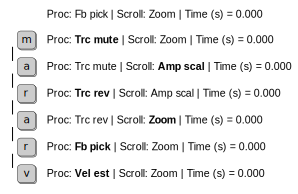
\includegraphics[width=.75\textwidth]{figures/status_bar.pdf}
	\caption{The status bar in the interactive seismogram plot displays the currently active processing and data scaling modes as well as the time (in seconds) at the current cursor position. By pressing the keys 'a', 'm', 'r', 'v' on the keyboard the different modes can be activated.}
	\label{fig:statusbar_intro}

\end{figure}

\DIFdelbegin \DIFdel{Through the }\texttt{\DIFdel{plot}} %DIFAUXCMD
\DIFdel{method the frequency spectrum of the currently selected trace data can be visualized:
}%DIFDELCMD < \newline
%DIFDELCMD < \includegraphics[width=.5\textwidth]{./figures/plot_spectrum.pdf}
%DIFDELCMD < \newline
%DIFDELCMD < %%%
\DIFdel{A frequency spectrum as shown in Figure~\ref{fig:spectrum} can be used to discriminate the dominating signal frequencies from those associated to the background noise, and thus allows for the definition of adequate filter settings.
}%DIFDELCMD < \begin{figure}
%DIFDELCMD < 	\centering
%DIFDELCMD < 	\includegraphics[width=.75\textwidth]{figures/spectrum.pdf}
%DIFDELCMD < 	%%%
%DIFDELCMD < \caption{%
{%DIFAUXCMD
\DIFdelFL{The frequency spectrum illustrates the frequency content of the currently selected traces, which allows for the identification of frequency ranges associated to noise, which can be omitted through the application of corresponding frequency filtering.}}
	%DIFAUXCMD
%DIFDELCMD < \label{fig:spectrum}
%DIFDELCMD < \end{figure}
%DIFDELCMD < %%%
\DIFdel{To improve the signal-to-noise ratio it is possible to apply filters on the selected traces through the }\texttt{\DIFdel{filter}} %DIFAUXCMD
\DIFdel{method, which utilizes the frequency filters implemented in the ObsPy package \mbox{%DIFAUXCMD
\citep[lowpass, highpass, bandpass and bandstop;][]{beyreuther2010}}\hskip0pt%DIFAUXCMD
, e.g.:
}%DIFDELCMD < \newline
%DIFDELCMD < \includegraphics[width=.5\textwidth]{./figures/filter.pdf}
%DIFDELCMD < \newline
%DIFDELCMD < %%%
\DIFdel{By default, filters are solely applied to the currently selected traces, yet setting the filter on hold allows the filtering of all subsequently selected traces with the same filter settings.
In case the seismogram plot is opened, the effect of the applied filter on the seismic waveforms is interactively visualized.
}%DIFDELCMD < 

%DIFDELCMD < %%%
\DIFdelend \subsubsection{Analysis of the seismic waveforms and first break traveltime picking}

In the seismogram plot, the waveforms can be analyzed and processed to obtain information about the subsurface conditions. Activating the velocity estimation mode ('Vel est') by pressing the 'v' key on the keyboard, enables the user to estimate velocities for different wave phases (e.g., originating from a refractor) by pressing the left mouse button and moving the cursor. Once the left mouse button is released, a line between the start and end point is drawn and labeled with the corresponding velocity (estimates can be deleted by clicking with the right mouse button).

If the processing mode 'Fb pick' is activated, picking of first break traveltimes is done individually by clicking with the left mouse button on the respective trace. Clicking again on the same trace will set the first break pick to the new location as there can only be one traveltime for each SIN-RIN pair; whereas clicking with the right mouse button deletes the pick. Alternatively, first break picks can be set for multiple traces by pressing the left mouse button and moving the cursor. 
Once the left mouse button is released, first break picks are defined at the intersections between the line and the seismograms. In the same way, multiple picks can be deleted if a line is drawn with the right mouse button pressed. The first break traveltimes determined in the seismogram plot are automatically written to the project database when the window is closed or another set of traces is loaded by pressing the 'left' or 'right' arrow keys on the keyboard. 

The traveltime diagram for the currently active pickset can be created through the \texttt{plot} method:
\DIFdelbegin %DIFDELCMD < \newline
%DIFDELCMD < \includegraphics[width=.5\textwidth]{./figures/plot_traveltimes.pdf}
%DIFDELCMD < \newline
%DIFDELCMD < %%%
\DIFdelend \DIFaddbegin \DIFmodbegin
\begin{lstlisting}[language=Python, firstnumber=20,alsolanguage=DIFcode]
%DIF > # Plot traveltime diagram
%DIF > srm.plot(type='traveltimes')
\end{lstlisting}
\DIFmodend
\DIFaddend Figure~\ref{fig:traveltimes_intro} presents an exemplary traveltime diagram, which is a common way to examine the quality of the first break picking. Such illustration of the traveltimes can be used to identify outliers or erroneous measurements, which are commonly associated to traveltimes with substantial deviations from those observed at adjacent stations such as the first break pick for the SIN-RIN pair (23, 11). Outliers can be removed by clicking on the \DIFdelbegin \DIFdel{corresponding symbol ('x') }\DIFdelend \DIFaddbegin \DIFadd{respective data point }\DIFaddend in the traveltime diagram, which is instantly synchronized with the project database. If the seismogram plot and the traveltime diagram are used side-by-side, changes made to the first break picks in one window will interactively trigger an update of the other one and vice versa.
\DIFdelbegin %DIFDELCMD < 

%DIFDELCMD < %%%
\DIFdelend 
\begin{figure}
	\centering
	\DIFdelbeginFL %DIFDELCMD < \includegraphics[width=.75\textwidth]{figures/traveltimes_intro.pdf}
%DIFDELCMD < 	%%%
\DIFdelendFL \DIFaddbeginFL \includegraphics[width=.75\textwidth]{figures/traveltimes_syn.pdf}
	\DIFaddendFL \caption{The traveltime diagram shows the first break traveltimes stored in the currently active pickset along the y axis (x symbols), where solid lines connect traveltimes assigned to a common shot. The sort order of the stations along the x axis reflects the geometry. Filled circles indicate stations with co-located shot and geophone (receiver), triangles refer to receiver stations (no shot) and stars refer to shot stations (no geophone).}
	\label{fig:traveltimes_intro}

\end{figure}
\DIFdelbegin %DIFDELCMD < 

%DIFDELCMD < %%%
\DIFdel{The }\texttt{\DIFdel{SeismicRefractionManager}} %DIFAUXCMD
\DIFdel{handles first break picks in picksets, which can be organized and manipulated through the }\texttt{\DIFdel{picksets}} %DIFAUXCMD
\DIFdel{method of the }\texttt{\DIFdel{SeismicRefractionManager}}%DIFAUXCMD
\DIFdel{:
}%DIFDELCMD < \newline
%DIFDELCMD < \includegraphics[width=.5\textwidth]{./figures/picksets.pdf}
%DIFDELCMD < \newline
%DIFDELCMD < %%%
\DIFdel{Calling the }\texttt{\DIFdel{pickset}} %DIFAUXCMD
\DIFdel{method without parameters shows the status of all picksets in the project. From the above use case, we see that by default, the pickset 'picks' is loaded and activated, i.e., modifications of first breaks are stored in this pickset . First break picks provided by another source (as udf file) can be imported from  }\textit{\DIFdel{03\_proc/picks}}%DIFAUXCMD
\DIFdel{.
For the first break picking, it is sufficient to keep only one pickset in the workflow, i. e., not required picksets can be unloaded. A pickset currently not loaded can be deleted permanently, i.e., the corresponding traveltimes are removed from the database. The }\texttt{\DIFdel{picksets}} %DIFAUXCMD
\DIFdel{method can also be used to load picksets from the database:
}%DIFDELCMD < \newline
%DIFDELCMD < \includegraphics[width=.5\textwidth]{./figures/load_picksets.pdf}
%DIFDELCMD < \newline
%DIFDELCMD < %%%
\DIFdel{When a pickset is loaded from the database, it does not become the active pickset automatically; whereas by using the parameter }\texttt{\DIFdel{use}} %DIFAUXCMD
\DIFdel{the corresponding pickset is loaded and also becomes the active pickset. The first break traveltimes of a pickset can be exported to an udf file that }\DIFdelend \DIFaddbegin \DIFadd{Once the user is satisfied with the quality of the first break traveltimes, the data points of the pickset can be exported in the unified data format, which is compatible with the pyGIMLi framework. In particular, the udf file }\DIFaddend is stored in \DIFdelbegin \textit{\DIFdel{03\_proc/picks}} %DIFAUXCMD
\DIFdel{subdirectory }\DIFdelend \DIFaddbegin \DIFadd{the subdirectory }\textit{\DIFadd{03\_proc/picks}} \DIFaddend with the current timestamp as suffix:
\DIFdelbegin %DIFDELCMD < \newline
%DIFDELCMD < \includegraphics[width=.5\textwidth]{./figures/export_pickset.pdf}
%DIFDELCMD < %%%
\DIFdelend \DIFaddbegin \DIFmodbegin
\begin{lstlisting}[language=Python, firstnumber=22,alsolanguage=DIFcode]
%DIF > # Export first break traveltimes
%DIF > srm.picksets(do='export', name='pick')
\end{lstlisting}
\DIFmodend
\begin{footnotesize}
\DIFmodbegin
\begin{DIFverbatim}[alsolanguage=DIFcode]
%DIF > INFO    : Pickset 'pick' saved to pick_20230303T140447.pck'
\end{DIFverbatim}
\DIFmodend
\end{footnotesize}
\DIFaddend 

\DIFdelbegin \section{\DIFdel{Exemplary use cases}}
%DIFAUXCMD
\addtocounter{section}{-1}%DIFAUXCMD
%DIFDELCMD < 

%DIFDELCMD < %%%
\DIFdelend \subsection{\DIFdelbegin \DIFdel{Modeling and use }\DIFdelend \DIFaddbegin \DIFadd{Expanding the capabilities }\DIFaddend of \DIFdelbegin \DIFdel{synthetic seismic waveform data}\DIFdelend \DIFaddbegin \DIFadd{the formikoj library}\DIFaddend }
\DIFdelbegin %DIFDELCMD < 

%DIFDELCMD < %%%
\DIFdel{To demonstrate the applicability of the }\texttt{\DIFdel{SeismicWaveformModeler}} %DIFAUXCMD
\DIFdel{class, we generate two synthetic seismic waveform datasets assuming two horizontal layers in a half-space without topography and an interface between these layers with a constant depth.
Table~\ref{tab:syndata} summarizes the parameterization used for the forward modeling of one dataset without noise (Dataset\_1) and another dataset containing random noise and systematic errors (Dataset\_2).
For the visualization of both synthetic datasets, we provide the corresponding geometry files to the }\texttt{\DIFdel{SeismicRefractionManager}} %DIFAUXCMD
\DIFdel{in order to have full control regarding data selection and processing capabilities. 
}%DIFDELCMD < 

%DIFDELCMD < %%%
\DIFdel{The synthetic seismic waveforms for SIN 24 of Dataset\_1 presented in Figure~\ref{fig:syndata_clean} reveal clear negative first onsets and allow the identification of crossover points, i.e., inflexion points between the first arrivals from the first layer (RIN 17 to 30) and the first onsets associated to the second layer (RIN 1 to 16 and RIN 31 to 48).
In contrast the signal-to-noise ratio of Dataset\_2 (see Figure~\ref{fig:syndata_noise}) is a function of the offset between shot and geophone position, i.e., traces farther away from the shot contain a higher level of random noise. 
Moreover, Dataset\_2 also contains systematic errors, where RIN 6 and 14 refer to broken geophones, and RIN 35 is an example for readings with a wrong polarity.
We believe that such synthetic datasets might be useful for investigating the effect of complex survey geometries on seismic data as well as the development and evaluation of processing strategies.
}%DIFDELCMD < \begin{table}[pos=h]
%DIFDELCMD <     %%%
%DIFDELCMD < \caption{%
{%DIFAUXCMD
\DIFdelFL{Measurement scheme and parameters provided in the yaml files used to create synthetic seismic waveform datasets with (Dataset\_1) and without added noise (Dataset\_2).}}
    %DIFAUXCMD
%DIFDELCMD < \centering
%DIFDELCMD <     \begin{tabular}{lcc}
%DIFDELCMD <         \toprule
%DIFDELCMD <         %%%
\textbf{\DIFdelFL{Measurement scheme}} %DIFAUXCMD
%DIFDELCMD < & & \\
%DIFDELCMD <         %%%
\DIFdelFL{Number of stations }%DIFDELCMD < & %%%
\DIFdelFL{48 }%DIFDELCMD < & \\
%DIFDELCMD <         %%%
\DIFdelFL{Station spacing }%DIFDELCMD < & %%%
\DIFdelFL{2\,m }%DIFDELCMD < & \\
%DIFDELCMD <         %%%
\DIFdelFL{Number of geophones }%DIFDELCMD < & %%%
\DIFdelFL{48 }%DIFDELCMD < & \\
%DIFDELCMD <         %%%
\DIFdelFL{Number of shots }%DIFDELCMD < & %%%
\DIFdelFL{48 }%DIFDELCMD < & \\
%DIFDELCMD <         \midrule
%DIFDELCMD <         %%%
\textbf{\DIFdelFL{Model}} %DIFAUXCMD
%DIFDELCMD < & %%%
\textit{\DIFdelFL{Layer 1}} %DIFAUXCMD
%DIFDELCMD < & %%%
\textit{\DIFdelFL{Layer 2}} %DIFAUXCMD
%DIFDELCMD < \\
%DIFDELCMD < 		%%%
\DIFdelFL{Thickness }%DIFDELCMD < & %%%
\DIFdelFL{3\,m }%DIFDELCMD < & %%%
\DIFdelFL{10\,m }%DIFDELCMD < \\
%DIFDELCMD <         %%%
\DIFdelFL{Velocity }%DIFDELCMD < & %%%
\DIFdelFL{750\,m/s }%DIFDELCMD < & %%%
\DIFdelFL{3000\,m/s }%DIFDELCMD < \\
%DIFDELCMD <         \midrule
%DIFDELCMD <         %%%
\textbf{\DIFdelFL{Dataset}} %DIFAUXCMD
%DIFDELCMD < & %%%
\textit{\DIFdelFL{Dataset\_1}} %DIFAUXCMD
%DIFDELCMD < & %%%
\textit{\DIFdelFL{Dataset\_2}} %DIFAUXCMD
%DIFDELCMD < \\
%DIFDELCMD < 		%%%
\DIFdelFL{Noise }%DIFDELCMD < & %%%
\DIFdelFL{False }%DIFDELCMD < & %%%
\DIFdelFL{True }%DIFDELCMD < \\
%DIFDELCMD < 		%%%
\DIFdelFL{Noise level }%DIFDELCMD < & %%%
\DIFdelFL{0 }%DIFDELCMD < & %%%
\DIFdelFL{1e-5 }%DIFDELCMD < \\
%DIFDELCMD < 		%%%
\DIFdelFL{Missing shots }%DIFDELCMD < & %%%
\DIFdelFL{False }%DIFDELCMD < & %%%
\DIFdelFL{True }%DIFDELCMD < \\
%DIFDELCMD < 		%%%
\DIFdelFL{Broken geophones }%DIFDELCMD < & %%%
\DIFdelFL{False }%DIFDELCMD < & %%%
\DIFdelFL{True }%DIFDELCMD < \\
%DIFDELCMD < 		%%%
\DIFdelFL{Wrong polarity }%DIFDELCMD < & %%%
\DIFdelFL{False }%DIFDELCMD < & %%%
\DIFdelFL{True }%DIFDELCMD < \\
%DIFDELCMD < 		\midrule
%DIFDELCMD < 		%%%
\textbf{\DIFdelFL{Wavelet}} %DIFAUXCMD
%DIFDELCMD < & & \\
%DIFDELCMD < 		%%%
\DIFdelFL{Length }%DIFDELCMD < & %%%
\DIFdelFL{1.024\,s }%DIFDELCMD < & \\
%DIFDELCMD < 		%%%
\DIFdelFL{Frequency }%DIFDELCMD < & %%%
\DIFdelFL{100\,Hz }%DIFDELCMD < & \\
%DIFDELCMD < 		%%%
\DIFdelFL{Sampling rate }%DIFDELCMD < & %%%
\DIFdelFL{2000\,Hz }%DIFDELCMD < & \\
%DIFDELCMD <         \bottomrule
%DIFDELCMD <     \end{tabular}
%DIFDELCMD <     \label{tab:syndata}
%DIFDELCMD < \end{table}
%DIFDELCMD < \begin{figure}
%DIFDELCMD < 	\centering
%DIFDELCMD < 	\includegraphics[width=.75\textwidth]{figures/syn_clean_sin24.pdf}
%DIFDELCMD < 	%%%
%DIFDELCMD < \caption{%
{%DIFAUXCMD
\DIFdelFL{Synthetic seismic waveform data without random or systematic errors created with the }\texttt{\DIFdelFL{SeismicWaveformModeler()}} %DIFAUXCMD
\DIFdelFL{class for a shot position in the center of the survey layout.}}
	%DIFAUXCMD
%DIFDELCMD < \label{fig:syndata_clean}
%DIFDELCMD < \end{figure}
%DIFDELCMD < 

%DIFDELCMD < \begin{figure}
%DIFDELCMD < 	\centering
%DIFDELCMD < 	\includegraphics[width=.75\textwidth]{figures/syn_noise_sin24.pdf}
%DIFDELCMD < 	%%%
%DIFDELCMD < \caption{%
{%DIFAUXCMD
\DIFdelFL{Synthetic seismic waveform data with added noise created with the }\texttt{\DIFdelFL{SeismicWaveformModeler()}} %DIFAUXCMD
\DIFdelFL{class for a shot position in the center of the survey layout. The random noise refers to an offset dependent decrease of the signal-to-noise ratio, while the systematic broken geophones and wrong polarity are systematic errors.}}
	%DIFAUXCMD
%DIFDELCMD < \label{fig:syndata_noise}
%DIFDELCMD < \end{figure}
%DIFDELCMD < 

%DIFDELCMD < %%%
\DIFdel{Accordingly, the concept of the formikoj library allows the implementation of supplementary functionalities. 
Such }\DIFdelend \DIFaddbegin \DIFadd{Making the formikoj library publicly available under an open-source license 
allows the addition of supplementary functionalities tailored for the specific requirements of the users.
The concept of formikoj suggest that such }\DIFaddend custom extensions should be implemented either as internal methods or as functions in the utilities module, which are then executed through the \texttt{compute} method\DIFdelbegin \DIFdel{with a custom keyword.
As an illustrative example, we implemented }\DIFdelend \DIFaddbegin \DIFadd{.
}

\DIFadd{We illustrate this possibility for customization by implementing }\DIFaddend a simplified version of an automatic first break picking algorithm \DIFaddbegin \DIFadd{based on the short- and long-time window average ratio (STA/LTA) method \mbox{%DIFAUXCMD
\citep{allen1978}}\hskip0pt%DIFAUXCMD
}\DIFaddend , which determines the traveltimes \DIFdelbegin \DIFdel{based on }\DIFdelend \DIFaddbegin \DIFadd{following }\DIFaddend the energy ratio \DIFdelbegin \DIFdel{method \mbox{%DIFAUXCMD
\citep[e.g.,][]{earle1994}}\hskip0pt%DIFAUXCMD
. The }\DIFdelend \DIFaddbegin \DIFadd{approach \mbox{%DIFAUXCMD
\citep[e.g.,][]{earle1994}}\hskip0pt%DIFAUXCMD
. In particular, our implementation computes the envelope $E\left(t\right)$ of the seismogram $s\left(t\right)$ as \mbox{%DIFAUXCMD
\citep[e.g.,][]{duan2020}
}\hskip0pt%DIFAUXCMD
}

\begin{equation}
	\DIFadd{E(t)=\left(s\left(t\right)^2+\tilde{s}\left(t\right)\right)^{1/2}\,,
	\label{eq:envelope}
}\end{equation}
\DIFadd{where $\tilde{s}\left(t\right)$ is the Hilbert transform of $s\left(t\right)$. The energy ratio $ER$ is then computed as $ER=STA/LTA$ with
}

\begin{equation}
	\DIFadd{STA\left(i\right)=\frac{1}{n_{STA}}\sum_{j=i-n_{STA}}^{i}E\left(j\right)\,,
	\label{eq:sta}
}\end{equation}
\DIFadd{and 
}

\begin{equation}
	\DIFadd{LTA\left(i\right)=\frac{1}{n_{LTA}}\sum_{j=i-n_{STA}}^{i}E\left(j\right)\,,
	\label{eq:lta}
}\end{equation}
\DIFadd{where $n_{STA}$ and $n_{LTA}$ refer to the number of data points in $E\left(t\right)$ considered for the short- and long-time windows, respectively. For this exemplary implementation we determine the first break traveltimes in the seismograms as the position of the maximum in the $ER$ function, which is automatically saved in the project database. 
}

\DIFadd{The autopicking }\DIFaddend algorithm is added to the \texttt{SeismicRefractionManager} in form of two internal methods\DIFaddbegin \\ \DIFaddend \texttt{\_manage\_autopicking} and \texttt{\_compute\_autopicks}, respectively. \DIFdelbegin \DIFdel{The autopicking process can be started by passing the new keyword }\DIFdelend \DIFaddbegin \DIFadd{To invoke the autopicking process we modified the }\texttt{\DIFadd{compute}} \DIFadd{method, which now accepts the custom-defined keyword }\DIFaddend \texttt{\DIFdelbegin \DIFdel{autopick}\DIFdelend \DIFaddbegin \DIFadd{autopicking}\DIFaddend }\DIFdelbegin \DIFdel{as the first parameter to the }\DIFdelend \DIFaddbegin \DIFadd{. Additionally, the autopicking requires values to be passed for the parameters }\DIFaddend \texttt{\DIFdelbegin \DIFdel{compute}\DIFdelend \DIFaddbegin \DIFadd{pick}\DIFaddend } \DIFdelbegin \DIFdel{method:
}%DIFDELCMD < \newline
%DIFDELCMD < \includegraphics[width=.5\textwidth]{./figures/autopicking.pdf}
%DIFDELCMD < \newline
%DIFDELCMD < %%%
\DIFdel{The second parameter defines whether traveltimes should be determined for the entire dataset (}\DIFdelend \DIFaddbegin \DIFadd{and }\texttt{\DIFadd{pickset}}\DIFadd{. The former accepts the values }\DIFaddend \texttt{all} \DIFdelbegin \DIFdel{) or solely }\DIFdelend \DIFaddbegin \DIFadd{or }\texttt{\DIFadd{cur}} \DIFadd{to determine first break traveltimes }\DIFaddend for \DIFaddbegin \DIFadd{all traces in the dataset or solely }\DIFaddend the currently selected traces\DIFdelbegin \DIFdel{(}\texttt{\DIFdel{cur}}%DIFAUXCMD
\DIFdel{). The third parameter provides }\DIFdelend \DIFaddbegin \DIFadd{, respectively. The latter defines }\DIFaddend the name of the \DIFdelbegin \DIFdel{corresponding pickset in the project database; thus, making the traveltimes available for visualization and processing with existing functionalities or further custom implementations. }\DIFdelend \DIFaddbegin \DIFadd{picksets in which the automatically determined traveltimes should be saved to. A typical use case involves conducting the autopicking and exporting the determined traveltimes:
}\DIFmodbegin
\begin{lstlisting}[language=Python, firstnumber=24,alsolanguage=DIFcode]
%DIF > # Automatically pick first break traveltimes
%DIF > srm.compute(do='autopicking', pick='all', pickset='autopicks')
%DIF > srm.picksets(do='export', name='autopicks')
\end{lstlisting}
\DIFmodend
\begin{footnotesize}
\DIFmodbegin
\begin{DIFverbatim}[alsolanguage=DIFcode]
%DIF > INFO    : Created new pickset 'autopicks'
%DIF > INFO    : Pickset 'autopicks' loaded
%DIF > INFO    : 'autopicks' set at active pickset
%DIF > Progress <==============================> 100.0% completed
%DIF > INFO    : Pickset 'autopicks' saved to autopicks_20230303T140834.pck
\end{DIFverbatim}
\DIFmodend
\end{footnotesize}
\DIFaddend 

\DIFdelbegin \subsection{\DIFdel{First break travel time picking for a 2D roll-along field data set: the Danube island example}}
%DIFAUXCMD
\addtocounter{subsection}{-1}%DIFAUXCMD
%DIFDELCMD < 

%DIFDELCMD < %%%
\DIFdel{The seismic data used in this example were collected at the Danube island (Vienna) in June 2021, using 48 geophones deployed with 2\,m spacing between them and shot locations located between the geophone positions. As illustrated }\DIFdelend \DIFaddbegin \DIFadd{In Figure~\ref{fig:pickcomp}, we compare the automatically determined first break picks with the forward modeled traveltimes computed above to allow for a basic evaluation of autopicking performance. The inset plot in Figure~\ref{fig:pickcomp} presents the histogram of the autopicked traveltimes, which shows that three traveltimes should be considered outliers, and thus are removed from the dataset. After the outlier removal the correlation coefficient between forward modeled and autopicked traveltimes is \num{0.99} suggesting that the implemented autopicking algorithm performs well for the synthetic seismic waveform data. However, the observed deviation from the perfect correlation (i.e., the 1:1 line }\DIFaddend in Figure~\DIFdelbegin \DIFdel{\ref{fig:map_danube}, }\DIFdelend \DIFaddbegin \DIFadd{\ref{fig:pickcomp}) indicates that autopicking and forward modeling algorithm might be sensitive to different seismic wave phases. Further improvements in terms of the autopicking process could incorporate, for example, machine learning approaches as the method proposed by \mbox{%DIFAUXCMD
\citet{duan2020}}\hskip0pt%DIFAUXCMD
, which can be easily implemented as an additional functionality in the }\texttt{\DIFadd{SeismicRefractionManager}}\DIFadd{. We point out here, that following the same procedure, the user can implement further autopicking algorithms as well as other data processing strategies and have a simple framework for the evaluation of their performance through the analysis of synthetic data (e.g., clean and contaminated with Gaussian noise).
}\begin{figure}
	\centering
	\includegraphics[width=.75\textwidth]{figures/pick_comparison.pdf}
	\caption{\DIFaddFL{Comparison of forward modeled synthetic and automatically picked first break traveltimes for the synthetic seismic waveform data created in this study.}}
	\label{fig:pickcomp}
\end{figure}

\section{\DIFadd{Application to field data: Processing a 3D seismic refraction dataset}}

\DIFadd{To demonstrate the applicability of the  }\texttt{\DIFadd{SeismicRefractionManager}} \DIFadd{for the processing of real field data, we present here the analysis and inversion inversion results for a seismic refraction survey conducted in a soda lake located in the Nationalpark Neusiedler See--Seewinkel close to Vienna.
The seismic survey aims at solving for the geometry of the confined aquifer below this soda lake with the required information referring to }\DIFaddend the \DIFdelbegin \DIFdel{survey geometry refers to a roll-along geometry, i. e., }\DIFdelend \DIFaddbegin \DIFadd{thickness of the aquifer and }\DIFaddend the \DIFdelbegin \DIFdel{geophone spread was moved along a profile with 50\% overlap yielding a total of five segments.
The objective of the survey was to define the contact between different sediments within the tertiary and quarternary deposits used to build the man-made Danube island.
Additionally, the survey aimed to identify lateral changes that might indicate the position of a fault, which has been inferred from sediments recovered from drillings.
}\DIFdelend \DIFaddbegin \DIFadd{depth of the groundwater table.
As presented in Figure~\ref{fig:map_sodalakes}, the seismic data were collected with 48 geophones deployed along the North-East to South-West oriented line, and 48 geophones along the North-West to South-East oriented line, with a spacing of }\qty{2}{m} \DIFadd{between the geophones. Shots were generated with an }\qty{8}{kg} \DIFadd{sledgehammer at the geophone positions as well as at positions along the diagonals to obtain a sufficient coverage.
}

\DIFaddend 
\begin{figure}
	\centering
	\DIFdelbeginFL %DIFDELCMD < \includegraphics[width=.75\textwidth]{./figures/map_danube.pdf}
%DIFDELCMD < 	%%%
\DIFdelendFL \DIFaddbeginFL \includegraphics[width=.75\textwidth]{./figures/map_sodalakes.pdf}
	\DIFaddendFL \caption{The \DIFdelbeginFL \DIFdelFL{Danube island }\DIFdelendFL \DIFaddbeginFL \DIFaddFL{soda lakes }\DIFaddendFL field dataset was collected \DIFdelbeginFL \DIFdelFL{along }\DIFdelendFL \DIFaddbeginFL \DIFaddFL{in }\DIFaddendFL a \DIFdelbeginFL \DIFdelFL{single line with a roll-along }\DIFdelendFL \DIFaddbeginFL \DIFaddFL{3D }\DIFaddendFL survey layout \DIFdelbeginFL \DIFdelFL{; the }\DIFdelendFL \DIFaddbeginFL \DIFaddFL{with stations (co-located geophones and shots indicated by }\DIFaddendFL filled \DIFdelbeginFL \DIFdelFL{triangles indicate the direction }\DIFdelendFL \DIFaddbeginFL \DIFaddFL{dots) deployed in form }\DIFaddendFL of \DIFdelbeginFL \DIFdelFL{the measurements}\DIFdelendFL \DIFaddbeginFL \DIFaddFL{a cross}\DIFaddendFL . \DIFdelbeginFL \DIFdelFL{The five segments have an overlap }\DIFdelendFL \DIFaddbeginFL \DIFaddFL{Additional shots (yellow stars) were conducted in from }\DIFaddendFL of \DIFdelbeginFL \DIFdelFL{50\% }\DIFdelendFL \DIFaddbeginFL \DIFaddFL{a cross rotated by 45° }\DIFaddendFL to \DIFdelbeginFL \DIFdelFL{ensure an adequate data }\DIFdelendFL \DIFaddbeginFL \DIFaddFL{increase the }\DIFaddendFL coverage \DIFdelbeginFL \DIFdelFL{along }\DIFdelendFL \DIFaddbeginFL \DIFaddFL{of }\DIFaddendFL the \DIFdelbeginFL \DIFdelFL{entire profile}\DIFdelendFL \DIFaddbeginFL \DIFaddFL{dataset}\DIFaddendFL .}
	\DIFdelbeginFL %DIFDELCMD < \label{fig:map_danube}
%DIFDELCMD < %%%
\DIFdelendFL \DIFaddbeginFL \label{fig:map_sodalakes}
\DIFaddendFL 
\end{figure}

\DIFdelbegin %DIFDELCMD < \begin{table}[pos=h]
%DIFDELCMD <    %%%
\DIFdelendFL \DIFaddbeginFL \DIFaddFL{As in case of the synthetic dataset presented above, the geometry file contains the coordinates of the survey stations, yet for the soda lake dataset 3D coordinates we provided as illustrated in Table~\ref{tab:3d_geometry}. 
Since geophones were not deployed at each survey station the column }\textbf{\DIFaddFL{Geo}} \DIFaddFL{contains the value 1 (True) for the first 96 stations and 0 (False) for the remaining \num{20} stations. 
}
\begin{table}
   \DIFaddendFL \caption{\DIFdelbeginFL \DIFdelFL{Extract }\DIFdelendFL \DIFaddbeginFL \DIFaddFL{Excerpt }\DIFaddendFL from the \DIFdelbeginFL \DIFdelFL{roll-along }\DIFdelendFL \DIFaddbeginFL \DIFaddFL{3D }\DIFaddendFL survey geometry file\DIFdelbeginFL \DIFdelFL{showing how the information regarding the first geophone assigns the traces in the shot files to the correct stations}\DIFdelendFL .}
    \centering
    \begin{tabular}{rrrcrrr}
        \toprule
        \textbf{x (m)} & \textbf{y (m)} & \textbf{z (m)} & \textbf{Geo} & \textbf{Shot} & \textbf{1st Geo} & \textbf{\# Geo} \\
        \midrule
        \DIFdelbeginFL \DIFdelFL{0.0 }\DIFdelendFL \DIFaddbeginFL \DIFaddFL{40336.056 }\DIFaddendFL & \DIFdelbeginFL \DIFdelFL{0.0 }\DIFdelendFL \DIFaddbeginFL \DIFaddFL{292470.692 }\DIFaddendFL & \DIFdelbeginFL \DIFdelFL{163.5 }\DIFdelendFL \DIFaddbeginFL \DIFaddFL{120.0 }\DIFaddendFL & 1 & \DIFdelbeginFL \DIFdelFL{-1 }%DIFDELCMD < & %%%
\DIFdelFL{-1 }%DIFDELCMD < & %%%
\DIFdelFL{-1 }%DIFDELCMD < \\
%DIFDELCMD <         %%%
\DIFdelFL{2.0 }%DIFDELCMD < & %%%
\DIFdelFL{0.0 }%DIFDELCMD < & %%%
\DIFdelFL{163.5 }%DIFDELCMD < & %%%
\DIFdelFL{0 }%DIFDELCMD < & %%%
\DIFdelendFL 1001	 & \DIFdelbeginFL \textbf{\DIFdelFL{1}} %DIFAUXCMD
\DIFdelendFL \DIFaddbeginFL \DIFaddFL{1 }\DIFaddendFL & \DIFdelbeginFL \DIFdelFL{48 }\DIFdelendFL \DIFaddbeginFL \DIFaddFL{96 }\DIFaddendFL \\
        \DIFdelbeginFL \DIFdelFL{\vdots }\DIFdelendFL \DIFaddbeginFL \DIFaddFL{40334.751 }\DIFaddendFL & \DIFdelbeginFL \DIFdelFL{\vdots }\DIFdelendFL \DIFaddbeginFL \DIFaddFL{292469.177 }\DIFaddendFL & \DIFdelbeginFL \DIFdelFL{\vdots }\DIFdelendFL \DIFaddbeginFL \DIFaddFL{120.0 }\DIFaddendFL & \DIFdelbeginFL \DIFdelFL{\vdots }\DIFdelendFL \DIFaddbeginFL \DIFaddFL{1 }\DIFaddendFL & \DIFdelbeginFL \DIFdelFL{\vdots }\DIFdelendFL \DIFaddbeginFL \DIFaddFL{1002 }\DIFaddendFL & 	\DIFdelbeginFL \DIFdelFL{\vdots }%DIFDELCMD < & %%%
\DIFdelFL{\vdots }%DIFDELCMD < \\
%DIFDELCMD <         %%%
\DIFdelFL{94.0 }%DIFDELCMD < & %%%
\DIFdelFL{0 }%DIFDELCMD < & %%%
\DIFdelFL{163.5 }%DIFDELCMD < & %%%
\DIFdelFL{0 }%DIFDELCMD < & %%%
\DIFdelFL{1024 }%DIFDELCMD < & %%%
\textbf{\DIFdelFL{1}} %DIFAUXCMD
%DIFDELCMD < & %%%
\DIFdelFL{48 }%DIFDELCMD < \\
%DIFDELCMD < 		%%%
\DIFdelFL{96.0 }%DIFDELCMD < & %%%
\DIFdelFL{0 }%DIFDELCMD < & %%%
\DIFdelFL{163.5 }%DIFDELCMD < & %%%
\DIFdelendFL 1 & \DIFdelbeginFL \DIFdelFL{-1 }%DIFDELCMD < & %%%
\DIFdelFL{-1 }%DIFDELCMD < & %%%
\DIFdelFL{-1 }\DIFdelendFL \DIFaddbeginFL \DIFaddFL{96 }\DIFaddendFL \\
        \DIFdelbeginFL \DIFdelFL{98.0 }%DIFDELCMD < & %%%
\DIFdelFL{0.0 }%DIFDELCMD < & %%%
\DIFdelFL{163.5 }%DIFDELCMD < & %%%
\DIFdelFL{0 }%DIFDELCMD < & %%%
\DIFdelFL{1037 }%DIFDELCMD < & %%%
\textbf{\DIFdelFL{25}} %DIFAUXCMD
%DIFDELCMD < & %%%
\DIFdelFL{48 }%DIFDELCMD < \\
%DIFDELCMD <         %%%
\DIFdelendFL \vdots & \vdots & \vdots & \vdots & \vdots & \vdots & \vdots \\
		\DIFdelbeginFL \DIFdelFL{194.0 }\DIFdelendFL \DIFaddbeginFL \DIFaddFL{40284.472 }\DIFaddendFL & \DIFdelbeginFL \DIFdelFL{0.0 }\DIFdelendFL \DIFaddbeginFL \DIFaddFL{292455.431 }\DIFaddendFL & \DIFdelbeginFL \DIFdelFL{163.5 }\DIFdelendFL \DIFaddbeginFL \DIFaddFL{120.0 }\DIFaddendFL & \DIFdelbeginFL \DIFdelFL{0 }\DIFdelendFL \DIFaddbeginFL \DIFaddFL{1 }\DIFaddendFL & \DIFdelbeginFL \DIFdelFL{1049 }\DIFdelendFL \DIFaddbeginFL \DIFaddFL{1058 }\DIFaddendFL & \DIFdelbeginFL \textbf{\DIFdelFL{25}} %DIFAUXCMD
\DIFdelendFL \DIFaddbeginFL \DIFaddFL{1 }\DIFaddendFL & \DIFdelbeginFL \DIFdelFL{48 }\DIFdelendFL \DIFaddbeginFL \DIFaddFL{96 }\DIFaddendFL \\
		\DIFdelbeginFL \DIFdelFL{196.0 }\DIFdelendFL \DIFaddbeginFL \DIFaddFL{40285.896 }\DIFaddendFL & \DIFdelbeginFL \DIFdelFL{0.0 }\DIFdelendFL \DIFaddbeginFL \DIFaddFL{292454.027 }\DIFaddendFL & \DIFdelbeginFL \DIFdelFL{163.5 }\DIFdelendFL \DIFaddbeginFL \DIFaddFL{120.0 }\DIFaddendFL & 1 & \DIFdelbeginFL \DIFdelFL{-1 }\DIFdelendFL \DIFaddbeginFL \DIFaddFL{1059 }\DIFaddendFL & \DIFdelbeginFL \DIFdelFL{-1 }%DIFDELCMD < & %%%
\DIFdelFL{-1 }%DIFDELCMD < \\        
%DIFDELCMD <         %%%
\DIFdelFL{198.0 }%DIFDELCMD < & %%%
\DIFdelFL{0.0 }%DIFDELCMD < & %%%
\DIFdelFL{163.5 }%DIFDELCMD < & %%%
\DIFdelFL{0 }%DIFDELCMD < & %%%
\DIFdelFL{1073 }%DIFDELCMD < & %%%
\textbf{\DIFdelFL{49}} %DIFAUXCMD
%DIFDELCMD < & %%%
\DIFdelFL{48 }%DIFDELCMD < \\
%DIFDELCMD <         %%%
\DIFdelFL{200.0 }%DIFDELCMD < & %%%
\DIFdelFL{0.0 }%DIFDELCMD < & %%%
\DIFdelFL{163.5 }%DIFDELCMD < & %%%
\DIFdelendFL 1 & \DIFdelbeginFL \DIFdelFL{-1 }%DIFDELCMD < & %%%
\DIFdelFL{-1 }%DIFDELCMD < & %%%
\DIFdelFL{-1 }\DIFdelendFL \DIFaddbeginFL \DIFaddFL{96 }\DIFaddendFL \\
        \DIFdelbeginFL \DIFdelFL{202.0 }%DIFDELCMD < & %%%
\DIFdelFL{0.0 }%DIFDELCMD < & %%%
\DIFdelFL{163.5 }%DIFDELCMD < & %%%
\DIFdelFL{0 }%DIFDELCMD < & %%%
\DIFdelFL{1050 }%DIFDELCMD < & %%%
\textbf{\DIFdelFL{25}} %DIFAUXCMD
%DIFDELCMD < & %%%
\DIFdelFL{48 }%DIFDELCMD < \\
%DIFDELCMD <         %%%
\DIFdelendFL \vdots & \vdots & \vdots & \vdots & \vdots & \vdots & \vdots \\
        \DIFdelbeginFL \DIFdelFL{286.0 }\DIFdelendFL \DIFaddbeginFL \DIFaddFL{40339.421 }\DIFaddendFL & \DIFdelbeginFL \DIFdelFL{0.0 }\DIFdelendFL \DIFaddbeginFL \DIFaddFL{292402.681 }\DIFaddendFL & \DIFdelbeginFL \DIFdelFL{163.5 }\DIFdelendFL \DIFaddbeginFL \DIFaddFL{120.0 }\DIFaddendFL & \DIFdelbeginFL \DIFdelFL{0 }\DIFdelendFL \DIFaddbeginFL \DIFaddFL{1 }\DIFaddendFL & \DIFdelbeginFL \DIFdelFL{1084 }\DIFdelendFL \DIFaddbeginFL \DIFaddFL{1096 }\DIFaddendFL & \DIFdelbeginFL \textbf{\DIFdelFL{49}} %DIFAUXCMD
%DIFDELCMD < & %%%
\DIFdelFL{48 }%DIFDELCMD < \\
%DIFDELCMD <         %%%
\DIFdelFL{288.0 }%DIFDELCMD < & %%%
\DIFdelFL{0.0 }%DIFDELCMD < & %%%
\DIFdelFL{163.5 }%DIFDELCMD < & %%%
\DIFdelendFL 1 & \DIFdelbeginFL \DIFdelFL{-1 }%DIFDELCMD < & %%%
\DIFdelFL{-1 }%DIFDELCMD < & %%%
\DIFdelFL{-1 }\DIFdelendFL \DIFaddbeginFL \DIFaddFL{96 }\DIFaddendFL \\
		\DIFdelbeginFL \DIFdelFL{290.0 }\DIFdelendFL \DIFaddbeginFL \DIFaddFL{40305.228 }\DIFaddendFL & \DIFdelbeginFL \DIFdelFL{0.0 }\DIFdelendFL \DIFaddbeginFL \DIFaddFL{292445.050 }\DIFaddendFL & \DIFdelbeginFL \DIFdelFL{163.5 }\DIFdelendFL \DIFaddbeginFL \DIFaddFL{120.0 }\DIFaddendFL & 0 & 1097 & \DIFdelbeginFL \textbf{\DIFdelFL{73}} %DIFAUXCMD
\DIFdelendFL \DIFaddbeginFL \DIFaddFL{1 }\DIFaddendFL & \DIFdelbeginFL \DIFdelFL{48 }\DIFdelendFL \DIFaddbeginFL \DIFaddFL{96 }\DIFaddendFL \\
        \vdots & \vdots & \vdots & \vdots & \vdots & \vdots & \vdots \\
        \DIFdelbeginFL \DIFdelFL{386.0 }\DIFdelendFL \DIFaddbeginFL \DIFaddFL{40265.415 }\DIFaddendFL & \DIFdelbeginFL \DIFdelFL{0.0 }\DIFdelendFL \DIFaddbeginFL \DIFaddFL{292431.957 }\DIFaddendFL & \DIFdelbeginFL \DIFdelFL{163.5 }\DIFdelendFL \DIFaddbeginFL \DIFaddFL{120.0 }\DIFaddendFL & 0 & \DIFdelbeginFL \DIFdelFL{1109 }\DIFdelendFL \DIFaddbeginFL \DIFaddFL{1115 }\DIFaddendFL & \DIFdelbeginFL \textbf{\DIFdelFL{73}} %DIFAUXCMD
%DIFDELCMD < & %%%
\DIFdelFL{48 }%DIFDELCMD < \\
%DIFDELCMD <         %%%
\DIFdelFL{388.0 }%DIFDELCMD < & %%%
\DIFdelFL{0.0 }%DIFDELCMD < & %%%
\DIFdelFL{163.5 }%DIFDELCMD < & %%%
\DIFdelendFL 1 & \DIFdelbeginFL \DIFdelFL{-1 }%DIFDELCMD < & %%%
\DIFdelFL{-1 }%DIFDELCMD < & %%%
\DIFdelFL{-1 }\DIFdelendFL \DIFaddbeginFL \DIFaddFL{96 }\DIFaddendFL \\
		\DIFdelbeginFL \DIFdelFL{390.0 }\DIFdelendFL \DIFaddbeginFL \DIFaddFL{40255.453 }\DIFaddendFL & \DIFdelbeginFL \DIFdelFL{0.0 }\DIFdelendFL \DIFaddbeginFL \DIFaddFL{292431.395 }\DIFaddendFL & \DIFdelbeginFL \DIFdelFL{163.5 }\DIFdelendFL \DIFaddbeginFL \DIFaddFL{120.0 }\DIFaddendFL & 0 & \DIFdelbeginFL \DIFdelFL{2025 }\DIFdelendFL \DIFaddbeginFL \DIFaddFL{1116 }\DIFaddendFL & \DIFdelbeginFL \textbf{\DIFdelFL{97}} %DIFAUXCMD
%DIFDELCMD < & %%%
\DIFdelFL{48 }%DIFDELCMD < \\
%DIFDELCMD < 		%%%
\DIFdelFL{\vdots }%DIFDELCMD < & %%%
\DIFdelFL{\vdots }%DIFDELCMD < & %%%
\DIFdelFL{\vdots }%DIFDELCMD < & %%%
\DIFdelFL{\vdots }%DIFDELCMD < & %%%
\DIFdelFL{\vdots }%DIFDELCMD < & %%%
\DIFdelFL{\vdots }%DIFDELCMD < & %%%
\DIFdelFL{\vdots }%DIFDELCMD < \\
%DIFDELCMD < 		%%%
\DIFdelFL{570.0 }%DIFDELCMD < & %%%
\DIFdelFL{0.0 }%DIFDELCMD < & %%%
\DIFdelFL{163.5 }%DIFDELCMD < & %%%
\DIFdelFL{0 }%DIFDELCMD < & %%%
\DIFdelFL{2048 }%DIFDELCMD < & %%%
\textbf{\DIFdelFL{97}} %DIFAUXCMD
%DIFDELCMD < & %%%
\DIFdelFL{48 }%DIFDELCMD < \\		
%DIFDELCMD < 		%%%
\DIFdelFL{572.0 }%DIFDELCMD < & %%%
\DIFdelFL{0.0 }%DIFDELCMD < & %%%
\DIFdelFL{163.5 }%DIFDELCMD < & %%%
\DIFdelendFL 1 & \DIFdelbeginFL \DIFdelFL{-1 }%DIFDELCMD < & %%%
\DIFdelFL{-1 }%DIFDELCMD < & %%%
\DIFdelFL{-1 }\DIFdelendFL \DIFaddbeginFL \DIFaddFL{96 }\DIFaddendFL \\
        \bottomrule
    \end{tabular}
    \DIFdelbeginFL %DIFDELCMD < \label{tab:rollalong_geometry}
%DIFDELCMD < %%%
\DIFdelendFL \DIFaddbeginFL \label{tab:3d_geometry}
\DIFaddendFL 
\end{table}
\DIFdelbegin %DIFDELCMD < 

%DIFDELCMD < %%%
\DIFdel{In the field, each segment was measured separately, yet for the processing all measurements are combined in a single profile. 
We can implement such measurement layout in a geometry file 
as illustrated in Table~\ref{tab:rollalong_geometry}. 
The key parameter is '1st Geo' as it indicates the first active geophone along the profile for each shot file. For the first segment in a roll-along survey geometry, the first active geophone is always geophone 1. Considering the number of geophones used in each segment, and an overlap of 50\%, the first geophone for segments two to five are 25, 49, 73 and 97, respectively.
}%DIFDELCMD < 

%DIFDELCMD < \begin{figure}
%DIFDELCMD < 	\centering
%DIFDELCMD < 	\includegraphics[width=.75\textwidth]{figures/danube_island_cos_lp120.pdf}
%DIFDELCMD < 	%%%
%DIFDELCMD < \caption{%
{%DIFAUXCMD
\DIFdelFL{The common offset stack computed for the Danube island dataset clearly showing a two-layered subsurface. The seismic velocities within the layer can be estimated from the gradient of the lines drawn along the corresponding first onsets of the seismic waves.}}
	%DIFAUXCMD
%DIFDELCMD < \label{fig:fieldcos}
%DIFDELCMD < \end{figure}
%DIFDELCMD < 

%DIFDELCMD < %%%
\DIFdelend Based on the shot files and the geometry file stored in the required directory structure the \texttt{SeismicRefractionManager} creates the project database\DIFdelbegin \DIFdel{.
A first illustration of the subsurface conditions can be obtained by computing a common offset stack (COS):
}%DIFDELCMD < \newline
%DIFDELCMD < \includegraphics[width=.5\textwidth]{./figures/plotcos_danube.pdf}
%DIFDELCMD < \newline
%DIFDELCMD < %%%
\DIFdel{The COS for the Danube island dataset presented in Figure~\ref{fig:fieldcos} shows first onsets for absolute offsets up to approximately 150\,m, which suggest a two-layered subsurface model. By using the velocity estimation functionality we can approximate the seismic velocity in the corresponding layers.
}%DIFDELCMD < 

%DIFDELCMD < %%%
\DIFdel{For the first break picking a set of traces is selected, filtered if necessary and visualized:
}%DIFDELCMD < \newline
%DIFDELCMD < \includegraphics[width=.5\textwidth]{./figures/plotsin99_danube.pdf}
%DIFDELCMD < \newline
%DIFDELCMD < %%%
\DIFdel{In this example, the trace data for SIN 99 are used, which refers to a shot position located in segment four. 
As can be seen in Figure~\ref{fig:rollalong_pickwindow}, the first onsets are easily identifiable despite the substantial seismic background noise at large offsets (RIN 73 to 90).
}%DIFDELCMD < \begin{figure}
%DIFDELCMD < 	\centering
%DIFDELCMD < 	\includegraphics[width=.75\textwidth]{figures/danube_island_sin99_lp120_picks_vd.pdf}
%DIFDELCMD < 	%%%
%DIFDELCMD < \caption{%
{%DIFAUXCMD
\DIFdelFL{Examplary seismic waveforms from the Danube island dataset shown for shot index number (SIN) 99 with a 120 Hz lowpass filter applied to suppress high frequency noise. The receiver index numbers (RIN) start at 73, thus indicating that the data were collected with a roll-along survey geometry.}}
	%DIFAUXCMD
%DIFDELCMD < \label{fig:rollalong_pickwindow}
%DIFDELCMD < \end{figure}
%DIFDELCMD < %%%
\DIFdel{A pseudosection provides an illustration of the corresponding apparent seismic velocity values computed from the picked traveltimes and the distance between shots and geophones:
}%DIFDELCMD < \newline
%DIFDELCMD < \includegraphics[width=.5\textwidth]{./figures/plotpseudosection_danube.pdf}
%DIFDELCMD < 

%DIFDELCMD < %%%
\DIFdel{In a pseudosection, as presented in Figure~\ref{fig:rollalong_pseudosection} for the Danube island dataset, the apparent velocity values are assigned to pseudolocations, with the corresponding x- and z-coordinates determined as the midpoint and as $1/3$ of the absolute offset between the shot and geophone, respectively.
Accordingly, such plot allows for the identification of outliers in the data, e.g., stark velocity contrasts for adjacent points, or systematic errors, e.g., velocities erroneously influenced by a single shot or receiver. The main assumption here is that the pseudosection should reveal smooth transitions between lateral and vertical neighbors, considering that the data were collected with gradual changes in the position of the source (i.e., hammer blow) and the receiver (i.e., geophone). The pseudosection will reveal large variations in case of abrupt changes in the topography or the geometry of the array, yet this can be taken into account by the user during the identification of outliers and possible systematic errors.
For the Danube island dataset, the pseudosection suggests an increase in the seismic velocity along profile direction in deeper subsurface regions (i.e., larger pseudodepth). Such pattern could be related to a fault expected in this area of the Danube island, thus indicating that the geophysical survey was sufficiently designed to detect such feature.
Moreover, the pseudosection presented in Figure~\ref{fig:rollalong_pseudosection} shows a low number of data points in the first segment of the Danube island survey. This lack of data points at large pseudodepths is due to a low number of picked traveltimes at large offsets, and thus might indicate a low signal-noise ratio.
}%DIFDELCMD < \begin{figure}
%DIFDELCMD < 	\centering
%DIFDELCMD < 	\includegraphics[width=.75\textwidth]{figures/rollalong_pseudosection.pdf}
%DIFDELCMD < 	%%%
%DIFDELCMD < \caption{%
{%DIFAUXCMD
\DIFdelFL{Pseudosection showing the apparent seismic velocities determined from the first break traveltimes obtained from the Danube island dataset and the corresponding absolute offset between the shot and receiver stations. The apparent velocity for each shot-receiver pair is illustrated at the corresponding midpoint and pseudodepth (1/3 of the absolute offset).}}
	%DIFAUXCMD
%DIFDELCMD < \label{fig:rollalong_pseudosection}
%DIFDELCMD < \end{figure}
%DIFDELCMD < 

%DIFDELCMD < %%%
\DIFdel{To review the data quality along the entire profile it is possible to visualize the picking percentage, i.e., the ratio of actually picked traveltimes and total number of SIN-RIN pairs:
}%DIFDELCMD < \newline
%DIFDELCMD < \includegraphics[width=.5\textwidth]{./figures/plot_pickperc_danube.pdf}
%DIFDELCMD < \newline
%DIFDELCMD < %%%
\DIFdel{Figure~\ref{fig:rollalong_pickperc} shows that the picking percentage is visualized separately for each SIN. In this way, a low picking percentage indicates shots affected by a low signal-to-noise ratio. For the Danube island dataset, the picking percentage is low in the first segment, which confirms the lack of datapoints observed in the pseudosection. Moreover, the picking percentage plot can be used to track the picking progress, for instance
if the traveltimes cannot be determined in one session or 
to identify single shots that might have been forgotten during the first break picking. Accordingly, it is advisable to check the picking percentage prior to exporting the traveltimes for the inversion.
}%DIFDELCMD < 

%DIFDELCMD < \begin{figure}
%DIFDELCMD < 	\centering
%DIFDELCMD < 	\includegraphics[width=.75\textwidth]{figures/rollalong_pickperc.pdf}
%DIFDELCMD < 	%%%
%DIFDELCMD < \caption{%
{%DIFAUXCMD
\DIFdelFL{Picking percentage for each shot in the Danube island roll-along dataset. Low values in the first third of the dataset indicate a low signal-to-noise ratio in the seismograms hindering the picking of first break traveltimes for each shot-receiver pair.}}
	%DIFAUXCMD
%DIFDELCMD < \label{fig:rollalong_pickperc}
%DIFDELCMD < \end{figure}
%DIFDELCMD < %%%
\subsection{\DIFdel{Processing of a 3D seismic refraction dataset: the soda lake example}}
%DIFAUXCMD
\addtocounter{subsection}{-1}%DIFAUXCMD
%DIFDELCMD < 

%DIFDELCMD < %%%
\DIFdel{The }\texttt{\DIFdel{SeismicRefractionManager}} %DIFAUXCMD
\DIFdel{allows also the visualization and processing of data collected with a }\DIFdelend \DIFaddbegin \DIFadd{, automatically infers the }\DIFaddend 3D survey layout \DIFdelbegin \DIFdel{. To illustrate these capabilities, we present in Figure~\ref{fig:map_sodalakes} the geometry of a }\DIFdelend \DIFaddbegin \DIFadd{from the }\DIFaddend 3D survey \DIFdelbegin \DIFdel{conducted in a soda lake located close to Vienna. The soda lake corresponds to quarternary sediments where capillary forces have developed a low permeable layer close to the surface (between 50 }\DIFdelend \DIFaddbegin \DIFadd{geometry, }\DIFaddend and \DIFdelbegin \DIFdel{100 cm) with a high clay and salt content.
The seismic survey aims to support the interpretation of the electrical and electromagnetic models obtained in a monitoring framework. 
Accordingly, the survey geometryshown in Figure~\ref{fig:map_sodalakes} was specified by previously conducted electrical measurements with electrodes arranged along two perpendicular lines. The seismic data were collected with 48 geophones deployed along the North-East to South-West oriented line, and 48 geophones along the North-West to South-East oriented line, with a spacing of 2\,m between the geophones. Shots were generated with an 8\,kg sledgehammer at the geophone positions as well as at positions along the diagonals.
}%DIFDELCMD < 

%DIFDELCMD < \begin{figure}
%DIFDELCMD < 	\centering
%DIFDELCMD < 	\includegraphics[width=.75\textwidth]{./figures/map_sodalakes.pdf}
%DIFDELCMD < 	%%%
%DIFDELCMD < \caption{%
{%DIFAUXCMD
\DIFdelFL{The soda lakes field dataset was collected in a 3D survey layout with stations (co-located geophones and shots indicated by filled dots) deployed in form of a cross. Additional shots (yellow stars) were conducted in from of a cross rotated by 45° to increase the coverage of the dataset.}}
	%DIFAUXCMD
%DIFDELCMD < \label{fig:map_sodalakes}
%DIFDELCMD < \end{figure}
%DIFDELCMD < 

%DIFDELCMD < %%%
\DIFdel{The geometry file contains the 3D coordinates for each shot or receiver station, and thus the}%DIFDELCMD < \\ %%%
\texttt{\DIFdel{SeismicRefractionManager}} 
%DIFAUXCMD
\DIFdel{automatically }\DIFdelend \DIFaddbegin \DIFadd{thus }\DIFaddend configures the project for 3D processing. \DIFdelbegin \DIFdel{Figure~\ref{fig:3d_pickwindow} presents the }\DIFdelend \DIFaddbegin \DIFadd{Then we can select seismograms the same way as for the synthetic data presented above. For this example we select }\DIFaddend seismic waveform data recorded for SIN 1, i.e., the shot position co-located with the first geophone (Station 01 in Figure~\ref{fig:map_sodalakes})\DIFdelbegin \DIFdel{. The }\DIFdelend \DIFaddbegin \DIFadd{:
}\DIFmodbegin
\begin{lstlisting}[language=Python, firstnumber=10,alsolanguage=DIFcode]
%DIF > # Select traces with receiver
%DIF > srm.select(by='sin', num=1)
\end{lstlisting}
\DIFmodend
\begin{footnotesize}
\DIFmodbegin
\begin{DIFverbatim}[alsolanguage=DIFcode]
%DIF > INFO    : 96 traces selected
\end{DIFverbatim}
\DIFmodend
\end{footnotesize}
\DIFadd{In Figure~\ref{fig:3d_pickwindow}, we can see that the }\DIFaddend data for RIN 1 to 48 appear familiar as the corresponding SIN-RIN layout refers to the one of conventional 2D profiles; whereas the seismic waveforms for RIN 49 to 96 show an entirely different pattern. To understand such visualization, we need to take into account that RIN 49 to 96 are deployed perpendicular to the direction of propagation of the wavefront originating from SIN 1. Accordingly, the observed curvature in the first onsets is due to the varying offset of the different SIN-RIN pairs.
\DIFdelbegin %DIFDELCMD < 

%DIFDELCMD < %%%
\DIFdelend \begin{figure}
	\centering
	\includegraphics[width=.75\textwidth]{figures/sodalakes_sin1_lp100_picks_vd.pdf}
	\caption{Examplary seismic waveforms from the soda lakes dataset shown for shot index number (SIN) 1 with a 100 Hz lowpass filter applied to suppress high frequency noise. The recorded seismic waveforms clearly reflect the geometry of the geophones with RIN 1 to 48 deployed along the direction of wave propagation, while RIN 49 to 96 are deployed perpendicular to the propagating wavefront.}
	\label{fig:3d_pickwindow}
\end{figure}

Due to the 3D survey geometry, a 2D pseudosection is not suitable \DIFdelbegin \DIFdel{to illustrate the apparent velocity values obtained from the picked }\DIFdelend \DIFaddbegin \DIFadd{for assessing the quality of the }\DIFaddend first break traveltimes. \DIFdelbegin \DIFdel{Hence}\DIFdelend \DIFaddbegin \DIFadd{However}\DIFaddend , the \texttt{SeismicRefractionManager} \DIFdelbegin \DIFdel{automatically switches to a }\DIFdelend \DIFaddbegin \DIFadd{project is configured for }\DIFaddend 3D \DIFdelbegin \DIFdel{representation where }\DIFdelend \DIFaddbegin \DIFadd{processing, and thus }\DIFaddend the apparent velocity values are illustrated in an interactive 3D pseudosection. This plot can be rotated and the image section can be zoomed and panned allowing the user to easily investigate the data quality for 3D geometries. Figure~\ref{fig:3d_pseudosection} shows a screenshot of the 3D pseudosection for the salt lake dataset; yet, such screenshot cannot reveal the full capabilities implemented in the \texttt{SeismicRefractionManger} for the interactive analysis and visualization of 3D pseudosections.
\begin{figure}
	\centering
	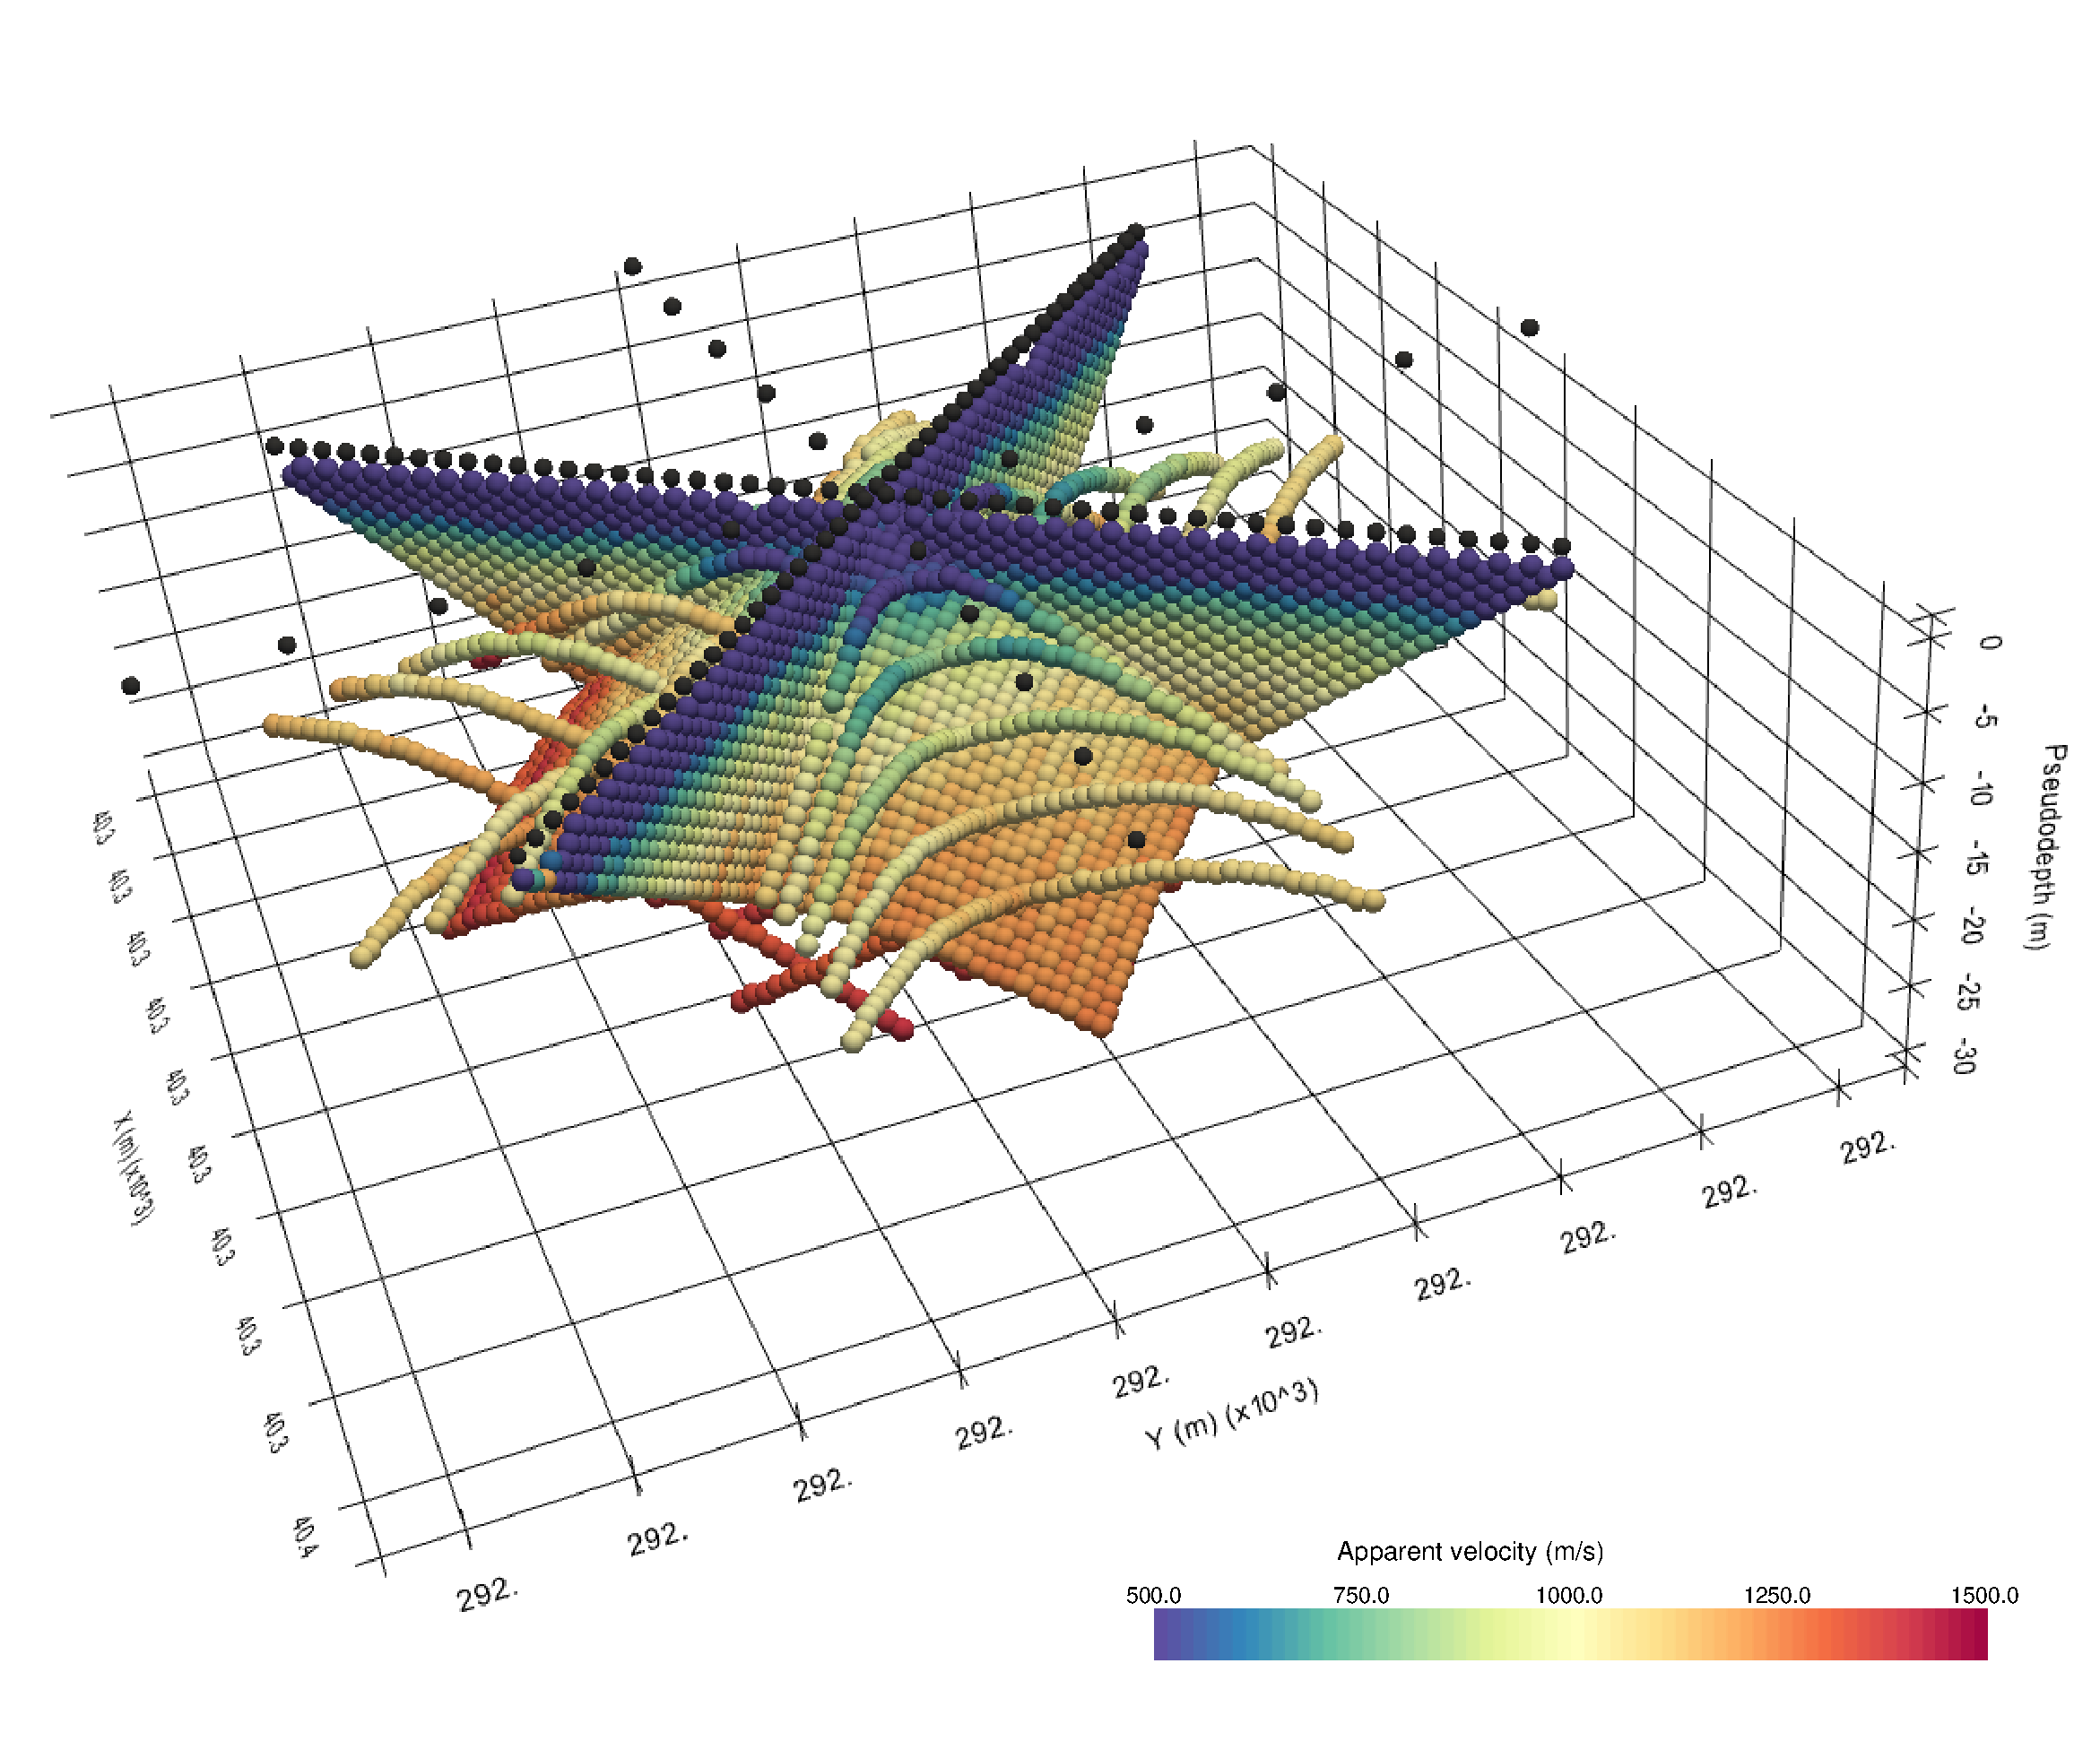
\includegraphics[width=.75\textwidth]{figures/3d_pseudosection.pdf}
	\caption{3D pseudosection showing the apparent seismic velocities determined from the first break traveltimes obtained from the soda lakes dataset and the corresponding absolute offset between the shot and receiver stations. The apparent velocity for each shot-receiver pair is illustrated at the corresponding 2D midpoint and pseudodepth (1/3 of the absolute offset), thus yielding a 3D representation.}
	\label{fig:3d_pseudosection}

\end{figure}

\DIFaddbegin \DIFadd{To review the data quality for the entire dataset it is possible to visualize the picking percentage, i.e., the ratio of actually picked traveltimes and total number of SIN-RIN pairs:
}\DIFmodbegin
\begin{lstlisting}[language=Python, firstnumber=10,alsolanguage=DIFcode]
%DIF > # Plot the picking percentage
%DIF > srm.plot(type='pickperc')
\end{lstlisting}
\DIFmodend
\DIFadd{Figure~\ref{fig:3d_pickperc} presents the picking percentage visualized separately for each SIN. Accordingly, a low picking percentage indicates shots affected by a low signal-to-noise ratio, whereas clear first onsets yield a correspondingly high picking percentage. For the soda lake dataset we observe a consistently high picking percentage for all shot positions; thus, indicating a good data quality.
Moreover, the picking percentage plot can be used to track the picking progress, for instance, in case the traveltimes cannot be determined in frame of one session or to identify single shots that might have been forgotten during the first break picking. Accordingly, it is advisable to check the picking percentage prior to exporting the traveltimes for the inversion.
}
\begin{figure}
	\centering
	\includegraphics[width=.75\textwidth]{figures/3d_pickperc.pdf}
	\caption{\DIFaddFL{Picking percentage for each shot in the soda lakes dataset indicating a high signal-to-noise ratio allowing for the picking of first break traveltimes for nearly all shot-receiver pairs.}}
	\label{fig:3d_pickperc}
\end{figure}

\DIFaddend Once the first break picking is finished, the corresponding pickset can be exported for the inversion. \DIFdelbegin \DIFdel{The inversion results and their interpretation are not }\DIFdelend \DIFaddbegin \DIFadd{We inverted the first break traveltimes with pyGIMLi and present the resolved 3D subsurface model in Figure~\ref{fig:3dinvres}a. From this representation we can see, that the inversion solves for low seismic velocities (\num{600} to }\qty{800}{ms^{-1}}\DIFadd{) in the near-surface in the center of the investigated area, which corresponds to the still intact part of the soda lake, i.e., the part that is covered by water on a seasonal basis. Seismic velocity values above }\qty{800}{ms^{-1}} \DIFadd{are resolved at depth as well as outside of the soda lake.
To facilitate the interpretation of the resolved seismic velocity distribution in terms of the aquifer geometry we show the two vertical slices in Figure~\ref{fig:3dinvres}b and c, respectively. In particular, we relate seismic velocity values $>\,$}\qty{800}{ms^{-1}} \DIFadd{to the transition from the unsaturated to the saturated zone due to the higher seismic velocity of water ($\approx\,$}\qty{1500}{ms^{-1}}\DIFadd{) compared to air ($\approx\,$}\qty{340}{ms^{-1}}\DIFadd{) filling the pore space. Accordingly, our 3D subsurface model indicates the depth of the groundwater table at a depth of approximately }\qty{8}{m}\DIFadd{. A more detailed interpretation is beyond }\DIFaddend the scope of this manuscript, yet \DIFdelbegin \DIFdel{Figures~\ref{fig:3d_pickwindow} and \ref{fig:3d_pseudosection} }\DIFdelend \DIFaddbegin \DIFadd{the presented figures }\DIFaddend reveal the capabilities provided by the proposed framework for the visualization and processing of data collected in 3D survey geometries.

\DIFaddbegin \begin{figure}
	\centering
	\includegraphics[width=.75\textwidth]{figures/inv_l100_ae0.0035.png}
	\caption{\DIFaddFL{Subsurface model of the soda lake in terms of the seismic P-wave velocity. (a) 3D representation of orthogonal slices through the resolved subsurface model. (b) 2D representation of the NE--SW slice. (c) 2D representation of the NW--SE slice.}}
	\label{fig:3dinvres}

\end{figure}

\DIFaddend \section{Conclusions and Outlook}

We have presented formikoj, a flexible open-source library enabling the development of modeling and processing tools for geophysical data. Implemented in python and tested on all major operating systems (Linux/Unix, MacOS, Windows), formikoj is suitable for multi- and cross-platform applications; thus, allowing collaboration between users free from licensing costs and platform requirements.

We demonstrated the capabilities of the formikoj framework to develop versatile and easily scalable classes for the modeling and processing of waveforms in seismic refraction surveys. \DIFdelbegin \DIFdel{The required interaction with the user is reduced to a minimum as }\DIFdelend \DIFaddbegin \DIFadd{By standardizing the data input in combination with a thorough sanity check aims at reducing the risk of corrupting the information stored in the project database.
Moreover, }\DIFaddend crucial processing steps are automatized within the \texttt{SeismicWaveformModeler} and \DIFaddbegin \DIFadd{the}\\ \DIFaddend \texttt{SeismicRefractionManager} \DIFdelbegin \DIFdel{based on }\DIFdelend \DIFaddbegin \DIFadd{classes facilitated by }\DIFaddend efficient data input strategies, for instance the preparation and import of the geometry file or the keyboard-based interaction related to the first break picking. In this regard, the user controls the formikoj library by providing text-based commands preferably through an ipython shell to exploit the full interactive potential modeling and processing tools. However, applications of the formikoj library can also be automatized by implementing workflows in python scripts or jupyter notebooks.

\DIFdelbegin \DIFdel{Based on three exemplary use cases, we illustrated the applicability of both the }\texttt{\DIFdel{SeismicWaveformModeler}} %DIFAUXCMD
\DIFdel{and the }\texttt{\DIFdel{SeismicRefractionManager}}%DIFAUXCMD
\DIFdel{. In the first use case, we showed the possibility to forward model seismic waveform data based on custom subsurface models and survey geometries with the }\texttt{\DIFdel{SeismicWaveformModeler}}%DIFAUXCMD
\DIFdel{. Additionally, the resulting waveforms can be subjected to systematic and random noise sources. 
The capabilities of the }\texttt{\DIFdel{SeismicRefractionManager}} %DIFAUXCMD
\DIFdel{were demonstrated through the processing of field datasets collected in complex survey layout, namely a roll-along and a 3D geometry. 
Moreover, we showed how the different data visualization options can assist during the data processing to ensure consistency in the first break traveltimes. In particular, we developed a visualization of the traveltimes by means of pseuodsections illustrating the corresponding apparent seismic velocities. Such plots allow for a quick identification of systematic errors and outliers in both 2D and 3D datasets.
}%DIFDELCMD < 

%DIFDELCMD < %%%
\DIFdelend By making the source code of the formikoj library available under the MIT license we intend to spark the development of further modeling and processing tools for various geophysical models based on this framework. Our further efforts will focus on implementing tools for other wave-based geophysical methods used in frame of our research activities, such as multi-channel analysis of (seismic) surface waves or magnetotelluric surveys. 

\section{Acknowledgments}

%The authors acknowledge TU Wien Bibliothek for financial support through its Open Access Funding Programme.
The authors are grateful to Nathalie Roser and Lukas Aigner for \DIFdelbegin \DIFdel{benchmarking }\DIFdelend \DIFaddbegin \DIFadd{using and testing }\DIFaddend the formikoj library \DIFdelbegin \DIFdel{against established software packages }\DIFdelend in frame of their research activities\DIFaddbegin \DIFadd{, and for providing valuable suggestions for improvement}\DIFaddend . Furthermore, we would like to thank Clemens Moser, Martin Mayr, Vinzenz Schichl and Harald Pammer for their constructive comments during first tests of the formikoj framework as well as for their help during the seismic surveys.

\newpage

\textbf{Code and data availability section}

Name of the code/library: formikoj

Contact: matthias.steiner@geo.tuwien.ac.at

Hardware requirements: No specific requirements

Program language: Python

Software required: Anaconda/Miniconda recommended

Total program and dataset size: 250 MB

The source codes and exemplary \DIFdelbegin \DIFdel{data sets }\DIFdelend \DIFaddbegin \DIFadd{datasets }\DIFaddend are available for downloading at the link:

https://git.geo.tuwien.ac.at/msteine1/formikoj.git

The \DIFdelbegin \DIFdel{orthophotos used in Figures~\ref{fig:map_danube} and \ref{fig:map_sodalakes} were }\DIFdelend \DIFaddbegin \DIFadd{orthophoto used in Figure~\ref{fig:map_sodalakes} was }\DIFaddend published by geoland.at under a CC BY 4.0 license.
\DIFaddbegin 

\appendix

\section{\DIFadd{Source code for generating the subsurface model considered in this study}}
\DIFmodbegin
\begin{lstlisting}[language=Python,alsolanguage=DIFcode]
%DIF > # Import required packages
%DIF > import numpy as np
%DIF > import pygimli as pg
%DIF > import pygimli.meshtools as mt
%DIF > 
%DIF > # Create the model geometry
%DIF > # - top layer
%DIF > top = mt.createPolygon([[0, 0], [94, 0], 
%DIF >                         [94, -3.5], [72, -3.5], 
%DIF >                         [20, -2], [0, -2]],
%DIF >                        isClosed=True, marker=1, area=0.1)
%DIF > 
%DIF > # - bottom layer
%DIF > bottom = mt.createPolygon([[0, -2], [20, -2], 
%DIF >                            [22, -6], [70, -6], 
%DIF >                            [72, -3.5], [94, -3.5], 
%DIF >                            [94, -10], [0, -10]],
%DIF >                           isClosed=True, marker=3, area=0.1)
%DIF > 
%DIF > # - anomaly/infill
%DIF > infill = mt.createPolygon([[20, -2], [72, -3.5], 
%DIF >                            [70, -6], [22, -6]],
%DIF >                           isClosed=True, marker=2, area=0.1)
%DIF > 
%DIF > geom = top + infill + bottom
%DIF > 
%DIF > # Define shot and receiver stations and create corresponding nodes
%DIF > nstats = 48
%DIF > spc = 2
%DIF > 
%DIF > stations = np.vstack((np.linspace(0, (nstats-1)*spc, nstats), 
%DIF >                       np.zeros(nstats))).T
%DIF > 
%DIF > for p in stations:
%DIF >     geom.createNode(p)
%DIF > 
%DIF > # Create mesh for the finite element modeling
%DIF > mesh = mt.createMesh(geom, quality=34)
%DIF > 
%DIF > # Save the mesh in the binary mesh format for later use 
%DIF > # with the SeismicWaveformModeler
%DIF > mesh.save('mesh.bms')
\end{lstlisting}
\DIFmodend
\DIFaddend 

\bibliographystyle{cas-model2-names}
\bibliography{references} 

\end{document}

